%!TEX root = ../Studienarbeit.tex

%!TEX root = ../Studienarbeit.tex


\section{Hardwarerealisierung}

Für einen optimalen Vertreibungseffekt werden verschiedene Aktoren im System verbaut. Die einzelnen Geräte werden alle über eine externe Energieversorgung, beziehungsweise Batterie betrieben. Bei der Wahl der Batterie, ist ein wichtiges Kriterium, wie lange das System ohne Energiezufuhr funktionsfähig bleibt.
\\
Dabei wurde berücksichtigt, wie viel das System im Normalverbrauch ohne Einschalten der Aktoren verbraucht. Eine grobe Schätzung ergab, dass das System ungefähr 10 $\pm$ 2 Watt pro Stunde verbrauchen würde. Aus diesem Grund fiel die Wahl auf eine 50 Ah Autobatterie von \textit{BlackMax} \cite{Autobatterie} gefallen. Diese Batterie bietet ausreichend Kapazität, um das System über zwei Tage mit Energie zu versorgen.
\\
Ein weiterer Entscheidungsgrund für die Autobatterie ist der Strombedarf der Geräte. Wie nachfolgend beschrieben, kann die Wasserpumpe im laufenden Zustand bis zu 16 Ampere Strom beziehen. Viele leichte und kleine Batterien könnten langfristig durch diese Belastung Schaden nehmen. Da Autobatterien eine hohe Belastungsgrenze haben und hohe Ströme ermöglichen, sind sie daher für den Prototypen besser geeignet.

Für die Unterbringung aller Teile wird eine 40x55x30 \ac{CM} große Aluminiumkiste verwendet. Die Aluminiumkiste ist witterungsbeständig, und die Wärmeentwicklung im Inneren kann weitestgehend vernachlässigt werden. Aluminium hat nämlich eine gute Temperaturleitfähigkeit und kann somit einen Wärmestau verhindern. Dabei ist auch der Empfehlung aus einem \textit{Autodesk Instructables}-Projekt folge geleistet worden. In diesem Projekt wurde eine bewegungsausgelöste "`Wasserpistole"' aufgebaut. Allerdings war bei dem \textit{Instructables}-Projekt eine Vertreibung von Rehen vorgesehen, die sonst die Rosen im Garten aufgegessen hätten. Das Ziel dieser Arbeit ist es aber Waschbären und andere Kleintiere zu vertreiben, daher sind hier noch weitere Aktoren eingebaut. Zudem ist das \textit{Instructables}-Projekt nicht autark und portable, da es mit Strom und Wasser mittels Hausanschluss versorgt worden ist. \cite{watergun_dude}

Die eingebauten Bauteile werden nachfolgend beschrieben.

\subsection{Blitzlicht}

Für den Einsatz eines Abschrecklichtes mit Blitzlichtfunktion werden zwei LED-Scheinwerfer der Marke \textit{NAIZY} verwendet. Die Scheinwerfer sind für den Einsatz als Erweiterungsleuchten für Geländefahrzeuge gedacht. Sie sind wasserdicht und für den Außeneinsatz geeignet. Mit 1600 Lumen und grellweißem Farbton erzielen sie einen hohen stroboskopischen Effekt, mit dem die Tiere abgeschreckt werden. Aufgrund dieser Charakteristiken und des geringen Energieverbrauchs von 18 Watt sind sie für das Abschrecksystem sehr gut geeignet. \cite{am_licht}

Die beiden LED-Scheinwerfer sind an den beiden oberen Ecken der Box befestigt. Sie werden mit Transistoren durch den Mikrocontroller gesteuert. Um einen Gewöhnungseffekt zu vermeiden, sind die Scheinwerfer mit 0,5 bis 10 Hz beschaltet. Die Frequenz und Schaltung der Scheinwerfer wird dynamisch angepasst. Im Schaltbild aus Abbildung \ref{diag:lights_diagram} wird die Verwendung eines MOSFET-Treiberbausteins erkennbar. Der Treiber ermöglicht das Beschalten der Scheinwerfer mit höherer Leistung, als es mit dem Arduino möglich wäre. Der Treiber verfügt über eine zusätzliche Masse-Leitung, die mit dem Arduino verbunden ist. Dadurch ist es möglich den Strom zu schalten, auch wenn der Signalgeber und \textit{DC-Out} nicht die selbe Masse haben. \cite{mosfets_am}

\begin{figure}[h]
    \centering
    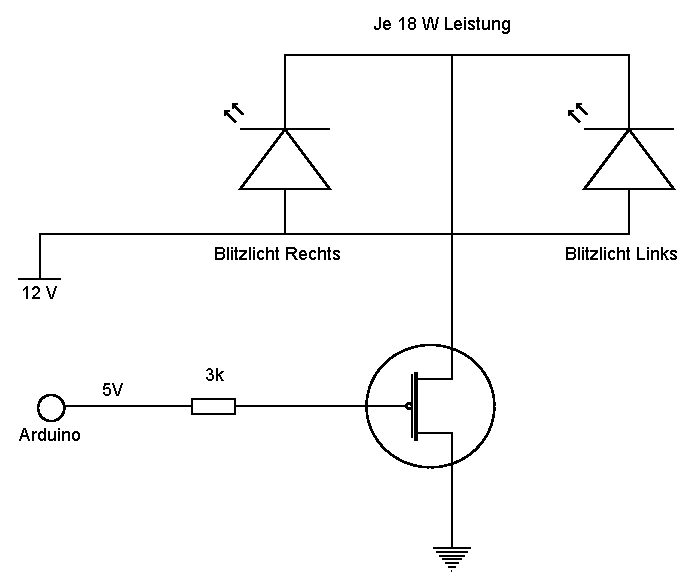
\includegraphics[width=0.6\textwidth]{images/lights_diagramm.pdf}
    \label{diag:lights_diagram}
    \caption{Schaltbild der Abschreckleuchten mit Ansteuerung}
\end{figure}

\subsection{Wasserversorgung und Pumpeneinheit}

Für den Einsatz eines \textit{Abschusssystems} mit Wasser benötigt das Abschrecksystem weitere Komponenten, welche folgend beschrieben werden.

\subsubsection{Pumpe} \label{cap:pumpe}

\comment{Bild mit Spritzschutz von Seite aus}

Auch wenn die Aluminiumkiste witterungsbeständig ist, schützt sie nur mäßig vor kalten Temperaturen. Dabei können viele Wasserpumpen schaden nehmen, wenn sie über den Winter draußen sind. Bei Membranpumpen ist dies ein kleineres Problem. Die zu den Oszillationsverdrängerpumpen gehörende Pumpenart ist außerdem sehr wartungsfreundlich und außerordentlich robust. Sie können daher selbst schwierigen Bedingungen und Temperaturumschwünge leicht standhalten.
\\
Ihre Funktionsweise beruht darauf, den \textit{Schöpfraum} periodisch zu vergrößern und zu verkleinern. Dadurch erzielen sie ihre Pumpwirkung und werden durch ihre Robustheit, Ölfreiheit (keine Verschmutzung der zu fördernde Flüssigkeit oder Gase) und Wartungsfreundlichkeit auch in chemischen Laboranwendungen verwendet. \cite{Jousten2018}

Für die Auswahl einer geeigneten Pumpe kamen zudem die Anforderungen an Fördermenge und Druck. Sprinkleranlagen werden wie in Kapitel \ref{sprinkler} beschrieben mit einem Gartenschlauch betrieben und können mit dieser Versorgung eine Reichweite von 10 Metern erreichen. Durch einen Hausanschluss fließen üblicherweise 20 Liter Wasser pro Minute mit einem Druck von etwa 4 Bar.\\
Die eingesetzte Pumpe von \textit{SEAFLO} hat eine maximale Fördermenge von 17 Liter pro Minute und kommt dadurch nahe an diesen Richtwert ran. Dabei nimmt sie bis zu 16 Ampere Strom auf. Auch bei dieser Leistungsaufnahme von über 190 Watt können die MOSFET-Treiber, die zum An- und Ausschalten der LED-Scheinwerfer verwendet werden, genutzt werden. Sie sind angegeben mit einer Dauerbelastung von 15 Ampere und mit Kühlung bis zu 30 Ampere. Da die Treiber nur für kurze Dauer eingeschaltet werden, ist eine zusätzliche Kühlung nicht nötig. \cite{mosfets_am,seaflo_pump}

Der Aufbau ist ähnlich zu dem Schaltbild \ref{diag:lights_diagram}. Allerdings wird zusätzlich eine Schutzdiode benötigt. Da Pumpen durch den internen Betrieb mittels Elektromotor eine induktive Last bilden, kann bei hartem Ein- und Ausschalten der MOSFET-Treiber durch Spannungsstöße Schaden nehmen \cite{induktive_last_diode}. Daher wird eine Schottky-Diode parallel zur Last eingebaut. Dies verhindert ein Aufbauen zu hoher Spannung, durch der der Transistor Schaden nehmen könnte. Schottky-Dioden eignen sich besonders gut für den Einsatz, da sie nur wenig Leistung aufnehmen und dadurch energiesparend sind. \cite{induktive_last_diode,am_schottky}

\subsubsection{Versorgung mit Wasser}

Damit die Pumpe mit Wasser versorgt werden kann, muss ein Wassertank in das System integriert sein. Allerdings ergeben sich dadurch verschiedene Probleme.
\\
Das größte Problem, das gelöst werden muss, ist die Unterbringung des Wassertanks. Durch den Einbau der verschiedenen Aktoren sowie der Autobatterie wurde in der Aluminiumkiste bereits viel Platz verwendet. Ein speziell an den verfügbaren Platz angepasster Tank kann zudem nicht mittels 3D-Drucker hergestellt werden, da die Drucke nicht wasserdicht sind. Ein herkömmlicher und einbaubarer Wassertank könnte daher nur wenige Liter fassen.

Ein weiteres Problem betrifft die Dichtigkeit des Tanks und der Pumpe. Beim Transport der Aluminiumkiste könnte eine große Menge Wasser leicht austreten. Aufgrund der Leitfähigkeit des Wassers könnten die Elektronikkomponenten Schaden nehmen. Dies wäre jedoch nicht so gravierend, da die Elektronik lediglich durchbrennen und der Stromkreislauf unterbrochen würde. Allerdings besteht bei der Aluminiumkiste die Gefahr, dass sie vollständig unter Strom gestellt wird. Dadurch würde sogar eine potenzielle Lebensgefahr entstehen, wenn man die Kiste berührt.
\\
Um die Sicherheit zu erhöhen, wird der Wassertank deshalb außerhalb der Kiste platziert und der Zulauf erfolgt durch eine seitliche Öffnung an der Kiste. Die Pumpe befindet sich jedoch weiterhin innerhalb der Kiste, um sie vor den äußeren Witterungsbedingungen zu schützen. Sie wird durch einen gedruckten Spritzschutz räumlich von den anderen Aktoren und der Spannungsversorgung getrennt. Der 3D-Druck ermöglicht jedoch keinen vollständigen Schutz, da er nur gegen geringe Wassermengen dicht hält. Spritzwasser und kleinere Leckagen durch die Pumpe können jedoch bewältigt werden.
\\
Vor dem Einbau in die Kiste wurde ein Dichtigkeitstest der Pumpe und des Spritzschutzes durchgeführt. Dabei traten nur bei bestimmten Bedingungen, wie dem seitlichen Legen oder Schütteln der Pumpe, geringe Mengen Wasser aus der Pumpe aus. Daher sollte der gedruckte Spritzschutz einen ausreichenden Schutz bieten.

\subsection{Mikrocontroller}

Durch die derzeitigen Liefermangel an Mikrocontrollern ergab sich die Auswahl eines passenden Mikrocontrollers für den Einsatz im Abschrecksystem ebenfalls als schwierig.\\
Getestet worden sind drei verschiedene Controller mit unterschiedlichen Erfolg, welche hier beschrieben werden.

Eine weitere Anforderung an das Abschrecksystem besteht darin, den Einsatz von \textit{Stereo Vision} für das korrekte Zielen zu ermöglichen. Alle drei Mikrocontroller sind daher mit zwei \ac{CSI}-Anschlüssen ausgestattet. Dies war von besonderer Bedeutung, da Multi-Camera Adapter wie von \textit{ArduCam} (\cite{arducam_multicam}) und auch USB-Kameras keine ausreichende Zeitsynchronität und Anpassbarkeit an das System ermöglichen. Nicht synchronisierte Kameras verfälschen die Tiefenberechnung sehr. Ein genaues Zielen wäre demnach nicht länger möglich wie aus der Arbeit von Shimizu und Co.hervorgeht. \cite{time_delay_sv}.
\\
Durch den direkten Anschluss an die \ac{CSI}-Anschlüsse wird dieses Delay minimiert. Die Mikrocontroller unterstützen teilweise die zeitgleiche Aufnahme von Bildern auf beiden \ac{CSI}-Anschlüssen. Im Falle des \textit{Jetson Nano}s ist eine Zeitsynchronität jedoch nicht vollständig gewährleistet. Dies geht aus dem \textit{ArduCam} Artikel von \cite{arduCam_sync_b01} hervor. Ein eigener Test ergab jedoch, dass die Kameras ausreichend synchron Bilder aufnehmen. Die Tiefenberechnung wäre demnach nicht zu stark beeinträchtigt, wie es mit dem \textit{MultiCam} Adapter der Fall wäre.

Um die Versorgungsspannung der 12V Autobatterie nutzen zu können, wird ein Spannungswandler benötigt, da die Mikrocontroller mit 5V betrieben werden. Der Spannungswandler muss in der Lage sein, kurzfristig eine ausreichende Leistung bereitzustellen. Bei der Objekterkennung können für einen kurzen Zeitraum hohe Leistungsabfragen entstehen. Wenn die Leistung dann nicht schnell genug bereitgestellt werden kann, kann es zum Zwangsabschaltungen des Mikrocontrollers kommen. Dadurch könnte auch der Controller selbst Schaden nehmen.
\\
Beim Aufsetzen und Testen des Jetson Nanos kam es wiederholt zu Stromabschaltungen. Der Nano wurde dabei mit einem Raspberry Pi Netzteil betrieben, das eine angegebene Leistung von 12,5 Watt hatte und daher für den Einsatz geeignet schien. Jedoch traten bei hohen Anforderungen, wie der gleichzeitigen Objekterkennung auf beiden Kameras, dennoch Stromabschaltungen auf. Im Gegensatz dazu traten beim Betrieb mit dem Spannungswandler und der Autobatterie keine unerwünschten Abschaltungen auf. Dies lag vermutlich daran, dass der einstellbare Spannungswandler von \textit{AzDelivery} laut den Angaben in \cite{am_spannungswandler} bis zu 60 Watt Leistung für den Mikrocontroller bereitstellen kann.

\subsubsection{Radxa \ac{CM} 3}

Durch den Liefermangel bestimmt waren Ende 2022 keine der nachfolgend beschrieben Mikrocontroller verfügbar. Daher ist das vom chinesischen Startup Radxa vertriebene \textit{Radxa Compute Module 3} für den Einsatz im Abschrecksystem getestet worden. Der Mikrocontroller zeichnet sich besonders durch die eingebaute \ac{NPU} sowie die verwendete Hardware wie \ac{SATA}-/USB 3.0-Anschlüsse und die Anzahl von 50 \ac{GPIO}-Pins aus. \cite{radxa}

Allerdings war das eigens für das \ac{CM} 3 konzipierte \textit{IO Board} zum Zeitpunkt der Untersuchung nicht erhältlich. Laut \textit{Radxa} ist das \ac{CM} 3 jedoch kompatibel mit dem \textit{\acl*{RPi} 4 IO Board}. Mit diesem Board kann das \ac{CM} 3 jedoch nur mit eingeschränkter Hardware genutzt werden.
\\
\textit{Radxa} bietet ein eigenes Betriebssystem für die Verwendung mit dem \ac{RPi} IO Board an. Bei der Einrichtung des Systems traten jedoch bereits Probleme auf. Zunächst konnte der \ac{eMMC}-Speicher nicht erfolgreich geflasht werden. Nur mit erhöhtem Aufwand war die Inbetriebnahme möglich.
\\
Im weiteren Betrieb traten weitere Probleme auf. Verschiedene Anwendungen und die Steuerung der Hardware (wie Kameras und \ac{GPIO}-Pins) waren sehr fehleranfällig und stürzten wiederholt ab.
\\
Auch konnte die \ac{NPU} des \ac{CM} 3 leider nicht mit den gängigen \ac{ML}-Frameworks wie Tensorflow genutzt werden. Stattdessen bietet \textit{Radxa} eine auf Linux basierende Toolchain an, um \ac{ML}-Projekte den Zugriff auf die \ac{NPU} zu ermöglichen. Die Einrichtung dieser Toolchain gestaltet sich jedoch als sehr umständlich, und viele Nutzer haben im \textit{Radxa}-Forum um Hilfe gebeten. \cite{radxa}

Aufgrund dieser Probleme konnte das \textit{Radxa Compute Module 3} nicht für das Abschrecksystem verwendet werden.

\subsubsection{Raspberry Pi \ac{CM} 3}

Auch \ac{RPi}-Geräte sind von Lieferengpässen betroffen. Die Geräte sind entweder nicht verfügbar oder nur zu überhöhten Preisen erhältlich. Glücklicherweise hatte das Unternehmen \textit{softwareinmotion} noch ein \ac{CM} 3+ auf Lager, dass für die Studienarbeit ausgeliehen werden konnte.
\\
Es ist jedoch zu beachten, dass das \ac{CM} 3 bereits veraltet ist, da seit 2020 das \ac{CM} 4 auf dem Markt ist. Der Hauptunterschied besteht darin, dass das \ac{CM} 3 mehr \ac{GPIO}-Pins hat, jedoch nur mit 1 GB DDR2 RAM erhältlich ist. Das \ac{CM} 4 hingegen verfügt über 1 bis 8 GB DDR4 RAM und ist mit USB 3.0 ausgestattet. \cite{cm4_cm3}

Die \ac{CM}-Mikrocontroller haben vor allem deshalb an Beliebtheit gewonnen, weil sie die Möglichkeit bieten, eigene Carrier Boards zu entwerfen. Diese Boards eröffnen neue Flexibilität, um die Hardware an spezifische Anforderungen anzupassen und maßgeschneiderte Lösungen zu entwickeln. Ein Beispiel dafür ist der \textit{StereoPi}, ein Carrier Board, der für die \ac{CM} Reihe entwickelt wurde. Der \textit{StereoPi} beschränkt Größe und Funktionalität des \acl{CM} auf die Stereo-Vision-Funktion, was ihn für bestimmte Anwendungen, wie die Tiefenberechnung besonders geeignet macht. Das \textit{StereoPi} Carrier Board hätte sich ideal für das Abschrecksystem geeignet. Bedauerlicherweise war es aufgrund der neuen Version und des Liefermangels nicht verfügbar, weshalb das standard Carrier Board von \acl{RPi} verwendet wurde. \cite{stereopi}

Der \ac{RPi} \ac{CM} 3+ ließ sich im Gegensatz zum \ac{CM} 3 von \textit{Radxa} problemlos in Betrieb nehmen. Allerdings ist es erforderlich, Jumper-Kabel an einige \ac{GPIO} Pins anzuschließen, um die Kameras nutzen zu können. Zudem müssen die Kameras über ein \ac{RPi} Zero Flachbandkabel mit dem \acs{CSI}-Anschluss am \ac{CM} verbunden werden. \cite{cm3}

Der \ac{CM} 3 Mikrocontroller eignet sich daher für den Betrieb, wurde jedoch aus anderen Gründen, die in Kapitel \ref{cap:Benchmarks} beschrieben sind, nicht verwendet.

\subsubsection{Nvidia Jetson Nano}

Der Jetson Nano Mikrocontroller hat eine ähnliche Größe und Form wie die Standard \ac{RPi}s. Im Vergleich zu den \ac{RPi}s verfügt der Jetson Nano jedoch nicht über WLAN oder Bluetooth. Dennoch besitzt er einen entscheidenden Unterschied: eine integrierte Grafikkarte. Aufgrund dieser Grafikkarte eignet sich der Jetson Nano besser für Aufgaben im Bereich des \acl{ML}s. \cite{nvidia_jn}

Grafikkarten (\acs{GPU}s) spielen eine essenzielle Rolle bei der Anwendung von \ac{ML} in der IT-Branche. SSie ermöglichen die parallele Verarbeitung von Daten und speziell Matrixoperationen. Diese Operationen werden in \ac{ML}-Algorithmen und \ac{DNN}s intensiv verwendet. Im Vergleich dazu können herkömmliche CPUs diese Operationen nur mit erheblichem Rechenaufwand bewältigen. Die hohe Rechenleistung und Parallelverarbeitungsfähigkeit von GPUs machen sie daher attraktiv bei \ac{ML}-Anwendungen. Auch ermöglichen sie eine verbesserte Manipulation und Auswertung von Bilddaten. Dies ist besonders vorteilhaft für das Abschrecksystem, da es in Echtzeit Bilder verarbeiten soll.
Die \ac{GPU}-basierte Verarbeitung kann dabei helfen, die Objekterkennung und Bewegungserfassung effizient auszuführen. Dadurch kann das Abschrecksystem schneller und präziser auf die Kleintiere reagieren. \cite{gpus}

Dennoch traten auch bei diesem Mikrocontroller Probleme auf, wie später in verschiedenen Kapiteln beschrieben wird. Der Jetson Nano hat sich jedoch aufgrund seiner Leistungsfähigkeit als \textit{"`Mini AI-Rechner"'} für das Abschrecksystem am besten geeignet.

\subsection{Sensorik-Kameras}

Viele unliebsame Kleintiere sind nachtaktiv. Daher muss das Abschrecksystem auch unter schwierigen Belichtungsbedingungen, insbesondere bei Nacht, die Kleintiere ebenso gut erkennen können wie bei Tageslicht. Aus diesem Grund ist es erforderlich, dass die eingesetzten Kameras eine Nachtsichtfunktion besitzen. Dafür werden infrarotsensible Kamerasensoren verwendet. Für den \acl{RPi} gibt es eine Variante der \textit{OV5647}-Kamera, die für diese Anwendung geeignet ist. Bei der "Nachtsicht"-Variante fehlt im Vergleich zur herkömmlichen Variante der Infrarotfilter. Im Tageslicht enthalten sind nämlich Infrarotstrahlen, die sonst für Rotstich-Aufnahmen sorgen. 
\\
Doch allein dadurch ist es noch nicht möglich, auch bei Nacht "`sehen"' zu können, da es nachts keine natürliche Infrarotstrahlung durch das Sonnenlicht gibt. Die Nachtsichtvariante der \textit{OV5647}-Kamera ist daher mit zwei zusätzlichen Infrarotstrahlern ausgestattet.
\\
Dadurch entsteht jedoch ein neues Problem: Rotstich-Aufnahmen führen sowohl tagsüber als auch nachts zu einer Verschlechterung der Bildqualität, was auch die Objekterkennung beeinträchtigen könnte. Um tagsüber keinen Rotstich zu erhalten, verfügt die \textit{OV5647}-Kamera über einen zuschaltbaren Infrarotfilter. Bei Nacht lässt sich der Rotstich dennoch nicht vollständig vermeiden. \cite{ov_5647}

Die Kamerasensoren sind jedoch nicht für den Jetson Nano geeignet, da laut einem Eintrag im Nvidia-Forum aus dem Jahr 2021 die Verarbeitung der reinen Kameradaten nicht öffentlich zugänglich ist. \cite{nvidia_forum_2021_nvidia}
\\
% Daher wurden \textit{IMX219}-Kamerasensoren in das Abschrecksystem eingebaut. Diese haben allerdings keinen zuschaltbaren Infrarotfilter, wodurch die Bilder besonders bei Tageslicht an Qualität verlieren, wie nachträglich in Kapitel \ref{cap:better_image} wird daher die Manipulation der Bilddaten nötig. Ein Vorher/Nachher-Effekt kann in Abbildung \ref{fig:better_image} betrachtet werden \cite{am_imx219}.


\section{Dreidimensionales Zielsystem} \label{cap:dreidim}

Für das dreidimensionale Zielsystem ergaben sich mehrere Herausforderungen. Einerseits musste eine präzise Steuerung des Zielsystems gewährleistet sein, andererseits musste die Reichweite von zehn Metern für den \textit{Wasserwerfer} erreicht werden.

Die präzise Steuerung ist insbesondere wichtig, da nur das anvisierte Ziel mit Wasser getroffen werden soll und nicht alles herum mit Wasser bespritzt wird. Dies ermöglicht es, Wasser nicht zu verschwenden und einen maximalen Vertreibungseffekt zu erzielen.
\\
In Tabelle \ref{tab:el_motors} sind einige Elektromotoren und ihre Vor- und Nachteile beschrieben. Die Elektromotoren eignen sich alle für den Einsatz im Zielsystem, haben aber Nebeneffekte, die bei der Auswahl mit berücksichtigt worden sind.
\\
Bei den Schrittmotoren stellte die präzise Ansteuerung ein Problem dar, da gängige Varianten nur eine Schrittweite von 1,9° haben. Dies würde zwar ausreichen, um größere Tiere gezielt anvisieren zu können, jedoch würde bei einer Entfernung von zehn Metern jeder Schritt eine Bewegung von 33 cm verursachen. Daher wäre ein Untersetzungsgetriebe erforderlich. Aufgrund des begrenzten Raums für das Zielsystem ist jedoch eine Implementierung eines solchen Getriebes nicht ohne weiteres möglich.
\\
Auch die DC-Elektromotoren konnten nicht verwendet werden, da auch ihr Einbau viel Platz erfordern würde. Um die Elektromotoren präzise auf eine bestimmte Position zu fahren, wären zudem Positionssensoren erforderlich. Sie müssten im Zielsystem verbaut werden und würden einen umfangreichen Aufbau erfordern. Darüber hinaus müssten für beide Motortypen zusätzliche Treiberplatinen beschafft und eingebaut werden, was die Kosten erhöhen und viel Platz in Anspruch nehmen würde.

Deshalb wurden kleine Servomotoren für das Zielsystem verwendet. Die eingebauten Servomotoren von \textit{Seamuing} sind normalerweise für den Einsatz in RC-Modellen vorgesehen, verfügen jedoch mit 245 N/cm über ein sehr hohes Drehmoment. Dieses Drehmoment wird benötigt, um den Gegenkräften des Wassers beim Zielen standzuhalten. Die Servos ermöglichen zudem eine präzise Auflösung von 0,09°. Somit wäre selbst im äußeren Zielbereich nur eine Abweichung von wenigen Zentimetern zu erwarten. Die Servos können zudem einfach über \ac{PWM} angesteuert werden, sind jedoch nur im Bereich von 0° bis 180° einstellbar. \cite{am_servos}

Die Servomotoren werden jedoch mit der im Modellbau üblichen Spannung von 7,4V betrieben. Hierfür eignet sich derselbe Spannungswandler, der auch für den Mikrocontroller verwendet wird. Bei dem verwendeten Spannungswandler kann nämlich die Ausgangsspannung über eine Stellschraube angepasst werden.

Die zweite Herausforderung bestand darin, die geeignete Wasserpumpe zu finden und einzustellen. Hierbei wurde, wie im Kapitel \ref{cap:pumpe} beschrieben, die Hausleitung und Sprinkleranlagen als Orientierung genutzt.
\\
Für die Zielberechnung wurde ebenfalls auf bestehende Sprinklersysteme zurückgegriffen. Deren Düsenöffnungen haben nur einen Durchmesser von wenigen Millimetern. Daher wurde der Durchmesser des "Laufs" auf zwei Millimeter verengt. Ein Test ergab, dass mit dieser Einstellung und der verwendeten \textit{SEAFLO} Pumpe eine Reichweite von 10 Metern erreicht werden kann.
\\
Dennoch muss für das präzise anvisieren die Flugbahn des Wassers bestimmt werden. Um die Berechnung zu vereinfachen wird die Formeln für den \textit{schrägen Wurf} angewendet, bei den äußere Bedingungen wie Luftwiderstand und Windgeschwindigkeit nicht beachtet werden. Dabei wird die Formel nach dem Startwinkel umgestellt. Die benötigten Parameter für die Berechnung sind dann die \textit{Anfangsgeschwindigkeit} sowie die \textit{x-} und \textit{y-}Koordinate des Ziels.
\\
Um die Formel anwenden zu können, fehlt nur noch die Anfangsgeschwindigkeit. Nachfolgend in Kapitel \ref{cap:calc_depth} ist, wie die \textit{x-} und \textit{y-} Koordinate bestimmt werden können.
\\
\begin{wrapfigure}{l}{0.4\textwidth}
    \centering
    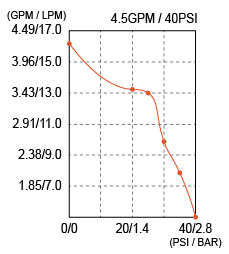
\includegraphics[width=0.35\textwidth]{images/seaflo_lpm_psi.png}
    \label{fig:psi_seaflo}
    \caption{Diagramm der Fördermenge gegenüber des Drucks. \cite{seaflo_pump}}
\end{wrapfigure}
Um die Anfangsgeschwindigkeit zu bestimmen, wurde zunächst angenommen, dass die Pumpe nahe ihrer maximalen Leistung betrieben wird. Diese Annahme basiert auf den Tests mit der zwei Millimeter Öffnung, bei denen auch die Druckabschaltung der Pumpe getestet wurde. Dabei wurde festgestellt, dass die Pumpe nahe der Druckabschaltung von etwa 2,8 Bar betrieben wird.
\\
Basierend auf dem Diagramm in Abbildung \ref{fig:psi_seaflo} lässt sich ableiten, dass die Pumpe bei dieser Einstellung eine Fördermenge von etwa 5 Litern pro Minute haben sollte. Mit diesen Daten kann die Austrittsgeschwindigkeit des Wassers berechnet werden. Dafür wird lediglich der Volumenstrom und der Querschnitt des Laufs benötigt. Allerdings ergibt die Formel $Geschwindigkeit = \frac{Volumenstrom}{Strömungsquerschnitt}$ aus \cite{stroemungen} keine korrekte Berechnung der Austrittsgeschwindigkeit, da ein Wert von über 265 Metern pro Sekunde berechnet wird. Es ist sehr wahrscheinlich, dass die Geschwindikeit durch den Luftwiderstand stark reduziert worden ist.
\\
Daher ist erneut die Formel für den \textit{schrägen Wurf} verwendet worden und nach der Anfangsgeschwindigkeit aufgelöst worden. Dabei stellte sich heraus, das die Anfangsgeschwindigkeit in etwa 10 Meter pro Sekunde beträgt.

Mit diesen Daten ist nun ein präzises anvisieren des Ziels möglich.

\subsection{Ansteuerung}

Zum Testen aller Funktionalitäten ist ein Arduino UNO verwendet worden. Der Arduino kann problemlos verwendet werden, um die Transistoren zu schalten und die Servomotoren zu steuern, da alle erforderlichen Bibliotheken bereits auf dem Board vorhanden sind. Der Testcode kann im Anhang unter \ref{list:Arduino_Test} eingesehen werden.
\\
Der Arduino schaltet alle Aktoren - Ton, Licht, Pumpe und Servomotoren - in bestimmten Zeitabständen ein und aus. Währenddessen werden die Servomotoren in inkrementellen Schritten angesteuert und ein Hochfrequenzton an zwei Pins ausgegeben. Bei diesen Tests stellte sich jedoch heraus, dass der erzeugte Ton zu leise war, um die Tiere effektiv zu stören. Daher wurde eine Verstärkerplatine hinzugefügt, die eine Ausgangsleistung von bis zu zehn Watt ermöglicht. Aus den Informationen von \cite{am_sound_amp} geht hervor, dass die Platine direkt ohne Spannungswandler von der Autobatterie mit Strom versorgt werden kann.
\\
Der Verstärker verfügt über einen Klinkenanschluss. Da der \textit{Jetson Nano} keinen Klinkenanschluss besitzt, wird ein USB-auf-Klinke-Adapter benötigt, um einen Ton abspielen zu können.

Der Jetson Nano besitzt 40 \ac{GPIO} Pins, mit denen die Transistoren geschaltet und die Servomotoren bedient werden können. Der Nano verfügt aber nur über zwei \ac{PWM} Pins. Eine Ansteuerung von mehr als zwei Servomotoren ist daher nicht möglich. \cite{jn_datasheet}

Das Steuern der Aktoren wird durch die von \textit{Nvidia} zur Verfügung gestellte \textit{Jetson.GPIO} Python Bibliothek ermöglicht. \cite{git_jn_gpio}
\\
Damit das Toggeln der Pins die Objekterkennung nicht blockiert, wurde eine threadbasierte Klasse erstellt, die jedem Pin einen eigenen Thread zuweist. Aus dem Hauptprogramm kann das Toggeln jederzeit durch den Befehl \textit{Pin.start\_toggle()} gestartet und durch \textit{Pin.stop()} pausiert werden. Auch kann die Frequenz des Toggelns durch das Multithreading dynamisch in dem Thread selbst verändert werden. Besonders für die Änderung der Schaltfrequenz für das Abschrecklicht eignet sich diese Funktion.
\\
Für die Steuerung der Servomotoren wurde eine ähnliche threadbasierte Klasse erstellt, bei der der Ansteuerungswinkel einfach und ähnlich wie im Arduino-Code aus \ref{list:Arduino_Test} angewendet werden kann.

Beim Testen der Toggle-Funktion wurde jedoch ein irreführendes Verhalten beobachtet. Das Schaltverhalten entsprach nicht immer den Vorgaben. Nach ausführlicher Fehlersuche und einen Blick in das Datenblatt des Jetson Nanos ergab, das die Spannung, die an den meisten \ac{GPIO} Pins anliegt, lediglich 1,8V beträgt und nur teilweise 3,3V. Die ausgewählten Transistortreiber sind jedoch für eine Schaltlogik von 3,3V bis 5V ausgelegt. Zudem wurde im Datenblatt der Transistoren festgestellt, dass bei Verwendung einer 3,3V-Logik der Strom auf unter 10 Ampere begrenzt werden sollte, da sich der Transistor sonst möglicherweise nicht abschalten lässt. Dieses Verhalten konnte beim Betrieb der Wasserpumpe festgestellt werden, da sie sich nur stark verzögert ausschaltete.
\\
Es traten noch weitere Probleme bei der Verwendung der \ac{PWM}-Steuerung der Servomotoren auf. Es schien, als ob die Servomotoren kein gültiges Signal vom Nano erhielten und keinerlei Bewegung zeigten. Bei der Messung der \ac{PWM} stellte sich heraus, dass keine \ac{PWM} erzeugt wurde. Selbst die Troubleshooting-Anleitungen von Nvidia brachten keine Lösung. In einigen Fällen wurde sogar versucht, wie von Nikola Jelic in \cite{forum_wrong_pwm} beschrieben, Registereinträge auf dem Nano vorzunehmen. Leider führten auch diese Versuche nicht zum gewünschten Erfolg. Daher muss für die Steuerung der Servomotoren eine alternative Lösung gefunden werden.
\\
Doch durch den Versuch die \ac{PWM} auf den Nano zu verwenden traten noch weitere Nebeneffekte auf. Das Toggeln der Pins war nicht mehr bis zum neustarten des Nanos möglich. Deshalb wurde die gesamte Hardwareansteuerung auf den Arduino UNO ausgelagert. Dieser hatte sich bereits durch den Funktionstest bewährt.

Für die Ansteuerung der Aktoren durch den Arduino wurde das Testprogramm aus \ref{list:Arduino_Test} angepasst. Der Arduino kann nun über den seriellen Port (USB) Befehle und Werte für die Steuerung des Zielsystems empfangen. Das Toggeln der Aktoren liegt vollständig in der Verantwortung des Arduino. Sobald er Werte für die Ansteuerung der Servomotoren erhält, wird er aktiv und steuert die Aktoren an. Die Steuerung wird solange ausgeführt, bis das Kommando "`g"' vom Nano empfangen wird. Das "`g"' steht dabei für \textit{gone} und signalisiert, dass das Ziel den Zielbereich verlassen hat.
\\
Auf der Seite des Jetson Nanos wurde außerdem eine threadbasierte Steuerung für den Arduino entwickelt. Die serielle Kommunikation mit dem Arduino benötigt deutlich mehr Zeit als die vorherige direkte Ansteuerung über die \ac{GPIO}-Pins, weshalb das Multithreading unbedingt erforderlich ist. Der Effekt auf die zeitliche Interferenz mit der Objekterkennung ist jedoch gering und es konnte keine signifikante Verbesserung durch das Multithreading festgestellt werden.

Den gesamten Schaltplan können Sie in Abbildung \ref{diag:all} einsehen. Die Kamerasensoren werden über den Jetson Nano betrieben und ihre Steuerung erfolgt hauptsächlich über Software. Daher werden sie erst in den nachfolgenden Kapiteln genauer beschrieben.

\begin{figure}[h]
    \centering
    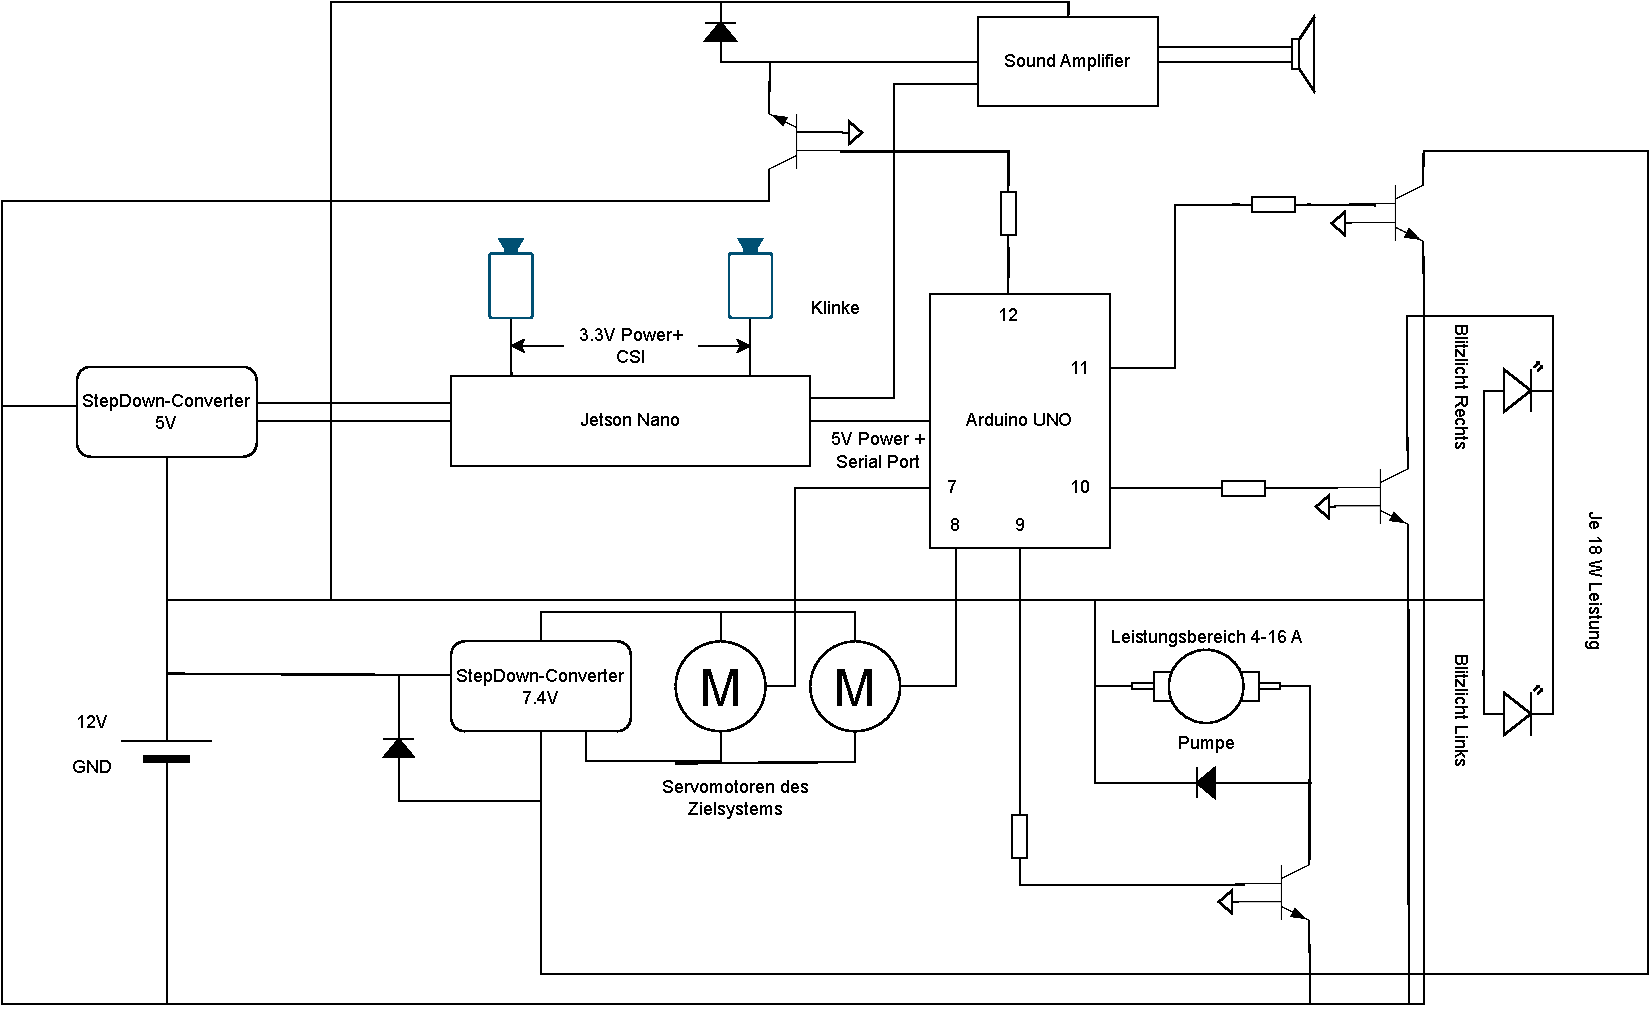
\includegraphics[angle=90,width=0.9\textwidth]{images/Schaltskizzen-Seite-3.drawio.pdf}
    \label{diag:all}
    \caption{Schaltplan der Hardware}
\end{figure}

\section{Objekterkennung und -Verarbeitung}

Der Haupteil der Arbeit bestand in der Entwicklung der Software, insbesondere der Implementierung der Objekterkennung und der Interaktion und Synchronisation der Kameras. Für das Training und Deployment der Objekterkennung wurden hauptsächlich Frameworks verwendet. Dennoch wurden auch einige Hilfsprogramme entwickelt und eingesetzt, welche im Folgenden beschrieben werden.

Für die Objekterkennung wurden verschiedene Modelle verwendet. Darunter zwei Modelle aus dem \textit{TensorFlow Model Zoo} und ein Modell von Google für ihren USB-Accelerator \textit{Coral}.
\\
Überwiegend wurde jedoch mit dem \textit{\ac{YOLO}v8}-Objekterkennungsmodell gearbeitet. Dieses Modell bot klare Vorteile gegenüber den anderen Frameworks. Insbesondere das sehr einfache Setup für das Training sowie die Exportmöglichkeit in verschiedene \ac{ML}-Formate überzeugten. Eine detaillierte Beschreibung dieser Vorteile wird im weiteren Verlauf gegeben.

\subsection{Ordner- und Datenstruktur} \label{cap:struktur}

TensorFlow bietet in \cite{tf2_object_detection_tut} ein eigenes Tutorial an, welches zeigt, wie man die Objekterkennung API nutzt und ein Objekterkennungsmodell trainiert und evaluiert. Diese Ordnerstruktur wurde für das Trainieren der Objekterkennungsmodelle übernommen und auf die eigene Nutzung angepasst. Die gesamte Ordnerstruktur ist in Abbildung \ref{fig:ordnerstruktur} zu sehen.

Aus der Struktur und dem Ablauf der Studienarbeit ergaben sich vier Kernbereiche, die auch in der Ordnerstruktur widergespiegelt werden. Das Projekt besteht aus den folgenden vier Ordnern: \verb|Dokumentation|, \verb|Dispositionspapier|, \verb|Deployment| und \verb|Detection_training| für das Training der Objekterkennung. Im folgenden werden aber nur die Inhalte des \verb|Deployment| und \verb|Detection_training| Ordners näher betrachtet.


\subsubsection{Deployment}

Der \textit{Deployment} Ordner enthält mehrere Unterordner, die zur besseren Übersicht und Einordnung der Funktionen dienen. Darunter befinden sich die \textit{Hardwareansteuerung}. Diese beinhalten auch die Arduino-Dateien des Funktionstestprogramms, sowie das Programm zur externen Steuerung des Zielsystems. Zudem ist in diesem Ordner das Python-Modul abgelegt, das die externe Ansteuerung des Arduinos ermöglicht.
\\
Das verworfene Python-Modul zur direkten Ansteuerung der Aktoren über die \ac{GPIO}-Pins des Jetson ist ebenfalls in diesem Ordner zu finden.

Des Weiteren gibt es einen separaten Ordner für die zeitlichen Inferenztests. In diesem Ordner befindet sich das Python-Skript, das die Ausführungszeit der verschiedenen Objekterkennungsmodelle und ihrer Formate testet. Die Auswertung der Inferenzzeit wird zudem in eine Markdown-Datei speichert.

Die weiteren Dateien, die in diesem Ordner abgelegt sind, werden in denen folgenden Kapiteln beschrieben.

{
\begin{wrapfigure}{l}{0.3\textwidth}
    \centering
    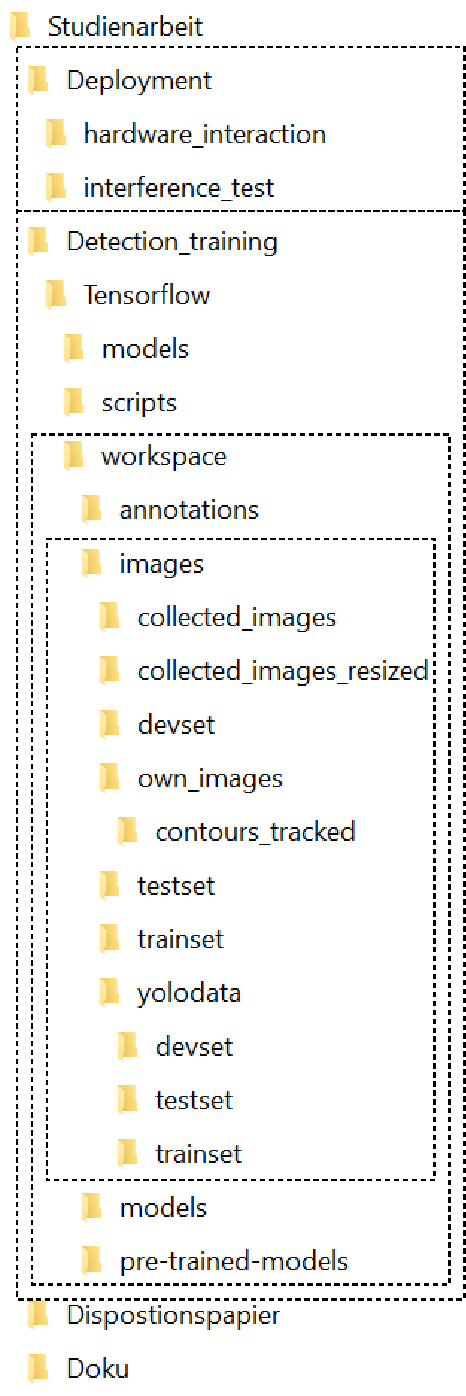
\includegraphics[width=0.28\textwidth]{images/ordner_struktur_with_lines.pdf}
    \label{fig:ordnerstruktur}
    \caption{Ordner-struktur des Projektes}
\end{wrapfigure}

\subsubsection{Detection training}

Im \verb|Detection_training| Ordner befinden sich zunächst die Jupyter-Notebooks für die Aufbereitung der Daten und der Auswertung der verschiedenen Modelle. Für die verschiedenen Trainingsmöglichkeiten sind jeweils eigene Notebooks erstellt worden.


Des Weiteren enthält der Ordner die modifizierte TensorFlow Ordnerstruktur. Darin befindet sich ein Skriptordner, welche einige Hilfsprogramme für das Trainieren der Objekterkennungsmodelle enthält. Die meisten dieser Hilfsprogramme sind jedoch für die Konvertierung der Bildannotationen in verschiedene Dateiformate zuständig.
\\
Der \textit{models} wird benötigt um die Objekterkennungs-API von TensorFlow nutzen zu können. In diesem sind die Installationsdateien, sowie Hilfsprogramme für die TensorFlow Objekterkennungs-API gespeichert.

Es ist auch von TensorFlow vorgesehen, Speicherorte für vortrainierte Objekterkennungsmodelle sowie für nachtrainierte oder selbst trainierte Modelle anzulegen. Diese werden im Unterordner \textit{workspace}.

Zusätzlich wird für das Trainieren mit TensorFlow eine Umwandlung der Bildannotationen in das TFRECORD-Format vorgesehen. Die konvertierten  Annotationen sind daher im \textit{annotations} Ordner unter dem \textit{workspace} Ordner zu finden.

}
Ein weiterer Unterordner des \textit{workspace} Ordner ist der \textit{images} Ordner, der alle Bilddaten enthält. Darin befindet sich ein Ordner mit der Bezeichnung \textit{collected\_images}. Er enthält alle Bilder und Annotationen, die für das Abschrecksystem verwendet wurden.


Zudem wird für das Trainieren der Modelle eine Zerteilung der annotierten Bilder in Train-, Test-, und Devset benötigt. Die Verteilung erfolgt mit den angegebenen Prozentsätzen: 85\% der Daten werden dem Trainingsset zugeordnet, 10\% dem Devset und 5\% dem Testset. Dadurch können die Modelle mit unterschiedlichen Datensätzen trainiert, validiert und getestet werden.
\\
Da \ac{YOLO} eine leicht veränderte Datenstruktur erwartet, wird diese separat im Unterordner \textit{yolodata} abgespeichert. Der Unterschied liegt dabei jedoch im Annotierungsformat.
\\
Für die Aufteilung werden die Daten aus dem \textit{collected\_images\_resized} Ordner entnommen. Der Ordner enthält alle Bilder und Annotationen, die auf eine einheitliche Höhe normiert wurden. Dies Normierung ist notwendig, da die Objekterkennungsmodelle bestimmte Bilddatenformate erwarten, wie beispielsweise 320x320 Pixel. Durch die Normierung der Bilder auf eine einheitliche Größe wird sichergestellt, dass während des Trainingsprozesses keine zusätzliche Zeit und RAM-Speicher für die Größenanpassung benötigt wird.
\\
Einige der Bilder im Originalformat haben eine hohe Auflösung, wie in etwa 4K-Qualität. Diese erfordern entsprechend viel Speicherplatz und erhöhen die Ausführungszeit während des Trainings. Durch die Umwandlung der Bilder von 4K auf 320x320 Pixel vor dem Training der Modelle wird der Speicherbedarf erheblich reduziert. Die Größe der Bilder nach der Umwandlung beträgt weniger als ein Prozent der ursprünglichen Größe. Dadurch wird eine schnellere Ausführung während des Trainingsprozesses ermöglicht und der Speicherplatzbedarf erheblich verringert.

Unter den Bildern befinden sich auch eigene Bilder, die vom Abschrecksystem selbst aufgenommen wurden. Sie sind im Ordner \textit{own\_images} gespeichert. Dabei wird auch unterschieden, ob es sich bei den aufgenommenen Bildern um erkannte Tiere handelt, die mittels Objekterkennung identifiziert wurden, oder ob es sich um eine Bewegungserkennung mittels Kontur-Tracking handelt. Die Disjunktion zwischen den beiden wird später beschrieben. 

\subsection{Sammlung der Trainingsdaten}

Zu Beginn der Arbeit wurde zunächst nach vergleichbaren Modellen und Datensätzen für die \textit{Objekterkennung} gesucht. Dabei fiel auf, dass es für einige unliebsame Kleintiere wie den \textit{Marder} leider keine geeigneten Datensätze gab.

Es gab jedoch bereits ein Modell für die Objekterkennung von Waschbären. Dat Tran hatte im Jahr 2017 ein TensorFlow-Lite-Modell für die Erkennung von Waschbären erstellt. Allerdings hatte er bei der Entwicklung eine andere Absicht. Die Tiere waren seine Lieblingstiere und er wollte wissen, wann ein Waschbär vor seiner Haustür auftaucht.
\cite{wasch_detect}

Mit etwas anderer Absicht lässt sich dies aber auch für die Studienarbeit nutzen, da Dat Tran seine 200 handgelabelten Bilder online zur Verfügung gestellt hat. Diese können für die Objekterkennung des Waschbären verwendet werden und dienen als Grundlage für das Training des Modells in der vorliegenden Arbeit.\\
Die Anzahl der Bilder erscheint für eine erste Betrachtung und Einarbeitung in das Trainieren eines eigenen Objekterkennungsmodells als geeignet. Ein Vergleich der Trainingsmodelle kann in Kapitel \ref{cap:Benchmarks} eingesehen werden.

Der Marder und der Waschbär waren aber nicht die einzigen Tiere, die aus dem Garten ferngehalten werden sollten. Auch Katzen, Füchse und Eichhörnchen sollten aus dem Garten ferngehalten werden. Die Absicht, Katzen und Eichhörnchen fernzuhalten, begründet sich damit, dass wir Vogelliebhaber sind und verhindern möchten, dass diese Tiere die Vögel stören oder ihnen schaden.
\\
Bei den Füchsen sieht es ähnlich aus. Sie sollen von den heimischen Beeten ferngehalten werden, da sie bekanntermaßen Krankheiten übertragen können und somit eine potenzielle Gefahr darstellen.

Um auch Marder und andere Tiere in die Erkennung aufzunehmen, wurden mehrere Datenlabeling-Programme getestet. Das Programm \textit{Label Studio} hat dabei am meisten überzeugt.
\\
\textit{Label Studio} bietet einen interaktiven Workflow und ermöglicht die Zusammenarbeit mehrerer Personen an einem Projekt. Tasks können verschiedenen Personen zugewiesen und übersichtlich dargestellt werden. Die benutzerfreundliche Drag-and-Drop-Oberfläche erleichtert das Labeln von Bildern und das Zeichnen von Bounding Boxes. Ein Beispiel für das Labeln eines Bildes wird in Abbildung \ref{fig:label_studio} exemplarisch dargestellt. Es ist jedoch zu beachten, dass das Bild bereits zu einem späteren Zeitpunkt der Studienarbeit stammt, bei dem das Abschrecksystem bereits funktionsfähig ist. \cite{labelstudio}

Die gelabelten Daten stehen anschließend in dem XML-basierten \textit{Pascal VOC} Datenanotierungsformat zur Verfügung.

\begin{figure}[H]
    \centering
    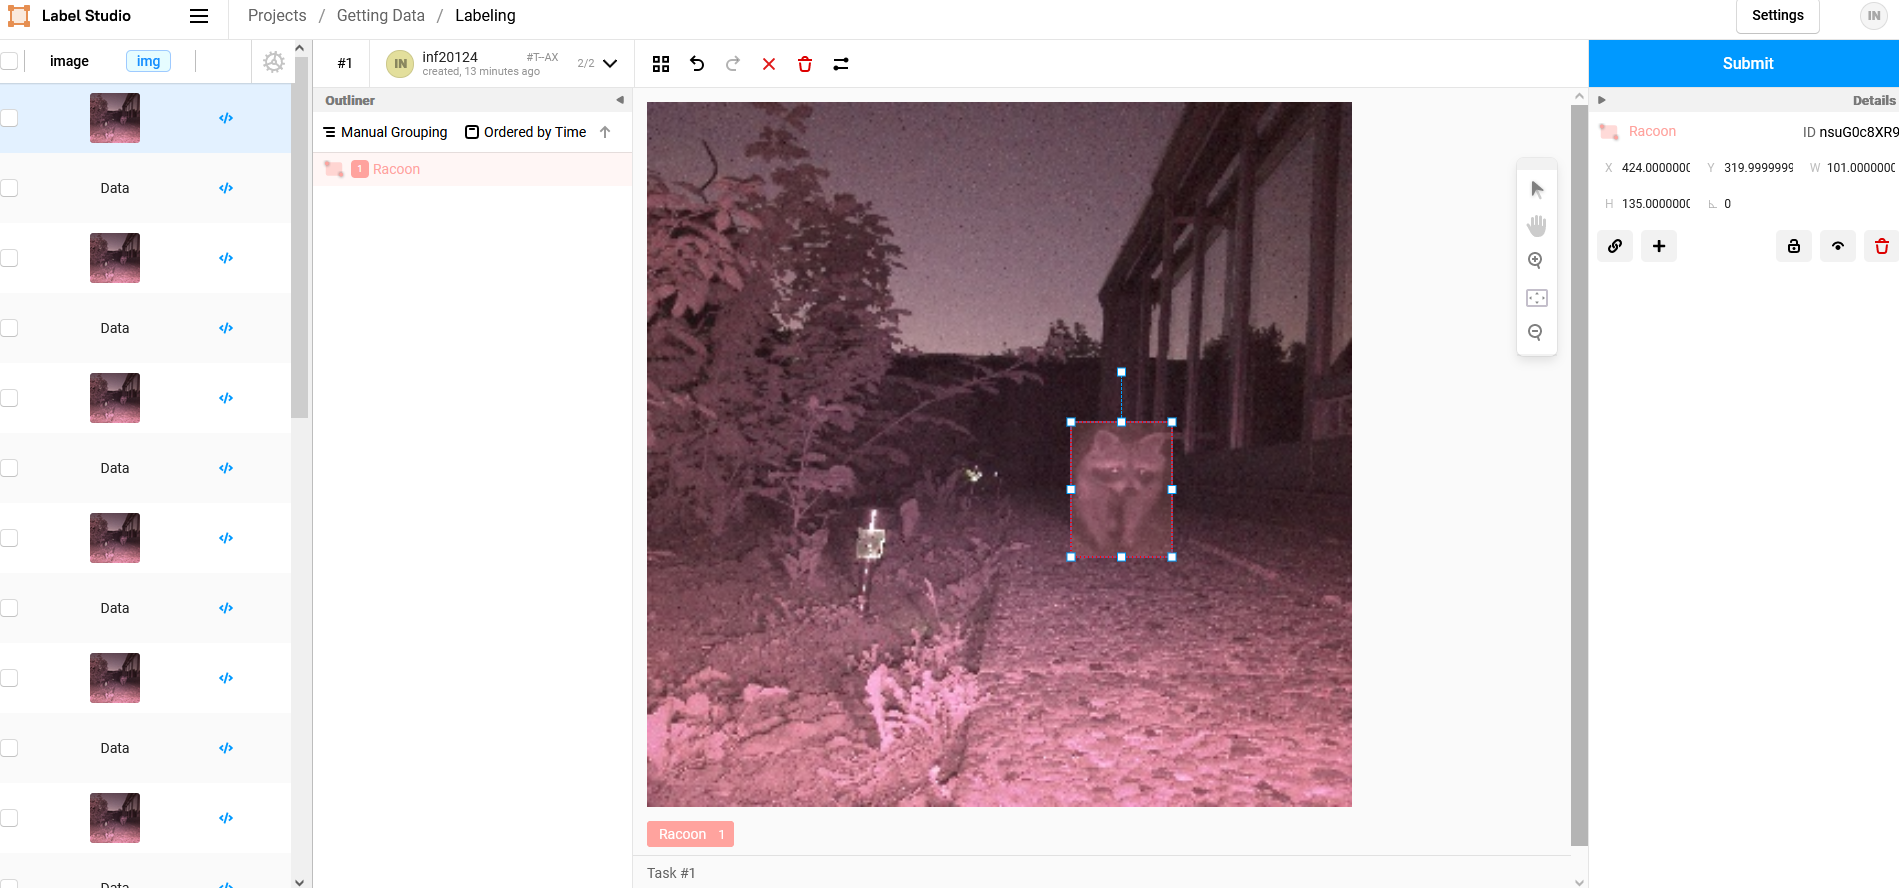
\includegraphics[width=\textwidth]{images/label_studio.png}
    \label{fig:label_studio}
    \caption{Einzeichnen einer Bounding Box mit dem Programm Label Studio}
\end{figure}

Das Problem beim manuellen Erstellen solcher Datensätze ist jedoch, dass dies viel Zeit in Anspruch nimmt. Ein ausreichend großer Datensatz kann daher innerhalb des vorgegebenen Zeitrahmens nicht erstellt werden. Aus diesem Grund wurde die Suche nach zusätzlichen Datensätzen erneut aufgenommen.
\\
Dabei stachen die Daten von \textit{Google Open-Images-V7} heraus. Der Datensatz enthält 16 Millionen Bounding Boxes auf 1,9 Millionen Bildern. Von den 600 verfügbaren Klassen sind auch die für die Arbeit relevanten Tiere enthalten. Allerdings ist ihre Verteilung ungleichmäßig. Ein Großteil der relevanten Bilder handelt von Katzen, während es weniger als tausend Bilder von Waschbären gibt. Daher ist zu erwarten, dass die Waschbären im Endprodukt schlechter erkannt werden als die Katzen. \cite{google_oi7}

Von den 1,9 Millionen Bildern in \textit{Google Open-Images-V7} sind nur etwa 17.000 für das Abschrecksystem relevant, da sie Waschbären, Katzen, Füchse oder Eichhörnchen enthalten. Nur diese Bilder sollten dem Datensatz hinzugefügt werden.
\\
Hier kommt \textit{FiftyOne} ins Spiel. \textit{FiftyOne} ist eine Open-Source-Bibliothek und Plattform zur Datenanalyse von Computer-Vision-Modellen. Eine Funktion von \textit{FiftyOne} ist das Extrahieren und Herunterladen von Computer-Vision-Datensätzen.
\\
Allerdings werden die Bilder und Bounding Boxes nicht getrennt von den nicht benötigten Daten heruntergeladen. Stattdessen werden CSV-Dateien heruntergeladen, die alle Bounding Boxes aufgeteilt in Train-, Test- und Devset enthalten. Diese CSV-Dateien werden anschließend von \textit{FiftyOne} ausgewertet, und die entsprechenden Bilder werden nachträglich heruntergeladen. \cite{fiftyone}

Das Herunterladen der Bilder kann je nach Bandbreite des Netzanbieters eine sehr lange Zeit in Anspruch nehmen. Besonders da die Größe der CSV-Datei, die alle Trainingsdaten beschreibt, bereits mehr als 2,1 GB groß ist. Zusätzlich zur Download-Zeit der CSV-Dateien kommt die Auswertungszeit hinzu, um festzustellen, welche Bilder heruntergeladen werden sollen, sowie die Download-Zeit der eigentlich ausgewählten Bilder.
\\
Nach dem Herunterladen der ausgewählten Bilder und den dazugehörigen Bounding Boxes steht der Datensatz immer noch nicht direkt zur Verwendung bereit. Die Bounding Boxes sind zwar vorhanden, jedoch sind sie weiterhin mit allen anderen Bounding Boxes kombiniert. Dabei beträgt die Größe der CSV-Datei für die Trainingsdaten 2,1 GB, was der Hälfte des Speicherplatzes der heruntergeladenen Bilddaten entspricht.
\\
Weitere Schritte sind daher erforderlich, um den Datensatz für das Training verwenden zu können. Unter dem Skriptordner ist daher ein in \textit{Rust} geschriebenes Konvertierungsprogramm mit der Bezeichnung \textit{csv\_conv} abgelegt. Dieses Skript konvertiert die heruntergeladenen CSV-Dateien in ein CSV-Format, das mit \textit{TensorFlow} kompatibel ist. Dabei werden auch alle nicht relevanten Bilddaten und Bounding Boxes herausgefiltert. Die Größe der resultierende CSV-Datei, die alle Trainings-, Test- und Devset-Bounding Boxes enthält, beträgt danach weniger als 1 MB.\\
Zusätzlich wurden irrelevante Daten entfernt, wie die Datenquelle sowie die Informationen \textit{IsOccluded, IsTruncated, IsGroupOf, IsDepiction, IsInside} und die \textit{Confidence}. Die \textit{Confidence} gibt an, mit welcher Wahrscheinlichkeit ein Objekt erkannt wurde. Jedoch spielt dieses Feld nur eine Rolle, wenn ein Objekterkennungsmodell die Bounding Box vorhersagen würde. Da dies bei den vorliegenden Daten nicht der Fall ist, kann das Feld ebenfalls gelöscht werden.
\\
Durch die Deserializierung können diese Felder automatisch ohne Mehraufwand in der Programmierung entfernt werden.
Als ein letzter Schritt werden danach die Bounding Box Daten, welche in Prozent angegeben sind, in eine Ganzzahl konvertiert und die Klasse des Objektes von einer ID zu einem Namen (zum Beispiel \textit{Racoon}) aufgelöst.

Nun gibt es jedoch ein weiteres Problem: Die Daten von Dat Tran und die von \textit{Google-Open-Images} liegen in unterschiedlichen Dateiannotierungsformaten vor. Allerdings hat Dat Tran in \cite{wasch_detect} bereits ein Python-Skript mit dem Namen \textit{xml\_to\_csv} erstellt, das die XML-Dateien in eine CSV-Datei konvertiert. Dieses Skript wurde an dieser Stelle verwendet und befindet sich ebenfalls im Skriptordner.

Mit den nun vorliegenden Daten kann die Objekterkennung angegangen werden.


\subsection{Bildmanipulation und -augmentation der gesammelten Bilder} \label{cap:augment}

Objekterkennungsmodelle lernen, Objekte anhand von Mustern, Farbtönen und Positionen im Vergleich zu anderen Objekten zu erkennen. Dies führt jedoch häufig zu "`Auswendiglernen'" oder Overfitting der Trainingsdaten. Wenn diese Modelle anschließend auf Daten angewendet werden, die nicht in den Trainingsdaten enthalten sind, können sie diese nur mit geringer Zuversichtlichkeit erkennen. Die Augmentierung der Trainingsdaten versucht, dieses Problem zu lösen, indem sie die Trainingsdaten manipuliert, um das Modell vielseitiger zu machen und unbekannte Daten besser zu erkennen.
\\
Gängige Möglichkeiten zur Durchführung von Bildmanipulationen sind:
\begin{itemize}
    \item Rotation der Bilder
    \item Ein- und Auszoomen der Bilder
    \item Abschneiden eines Bildteils
    \item Hinzufügen von zufälligem Jitter zu den Bildern
\end{itemize}
Es gibt jedoch viele weitere Möglichkeiten. Zum Beispiel bietet das TensorFlow-Framework 39 verschiedene Augmentierungsmöglichkeiten an. Auch andere Frameworks bieten ähnliche Möglichkeiten an. \cite{cv_Szeliski,tens_zoo}

Im vorherigen Abschnitt wurde beschrieben, wie die Daten für das Training der Modelle generiert wurden. Diese können jedoch nicht ohne weitere Anpassungen direkt für das Training verwendet werden, da sie nur geringfügig den erwartenden Bildern durch das Abschrecksystem entsprechen. Ein Beispiel dafür ist in Abbildung \ref{fig:vgl_img_data_real} dargestellt.

Links ist ein Bild aus dem Datensatz von Dat Tran zu sehen, während rechts ein Bild vom Abschrecksystem zu sehen ist. Die Bilder wurden bereits auf die gleiche Höhe normiert. Wie im vorherigen Kapitel \ref{cap:struktur} beschrieben, führt diese Bildmanipulation zu einer erheblichen Reduzierung der Zeit- und Ressourcenanforderungen während des Trainings.
\\
Die Größenanpassung selbst wird mithilfe eines Python-Skripts durchgeführt, das sich im Skriptordner befindet. Die Anpassung der Annotationen an die neue Bildgröße erfolgt mit einem separaten Rust-Programm.

\begin{figure}[H]
    \centering
    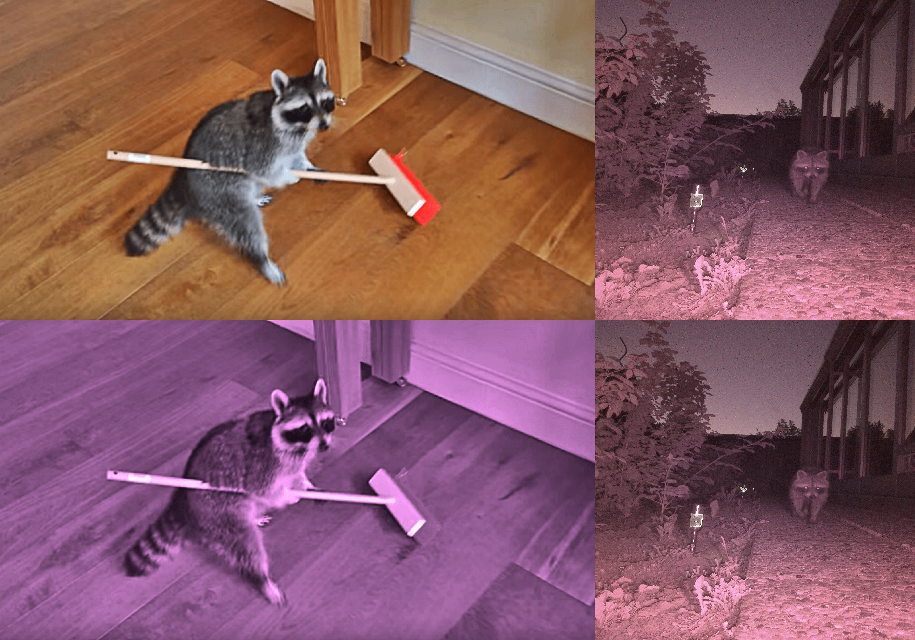
\includegraphics[width=\textwidth]{images/combine_augment.png}
    \label{fig:vgl_img_data_real}
    \caption{Vergleich eines augmentierten und nicht augmentierten Bildes aus den Trainingsdaten (links \cite{wasch_detect}) und ein Bild das vom Abschrecksystem aufgenommen wurde}
\end{figure}

Die verschiedenen Frameworks, die für das Training der Modelle verwendet werden, verfügen über diese Augmentierungsmöglichkeiten, die Trainingsbilder an die tatsächlichen Bilder anzugleichen. Dazu gehören manuelle Anpassungen an den Farbwerten, der Sättigung und der Dunkelstufe (HSV) an den einzelnen Bildern. In den jeweiligen Frameworks können diese verwendet werden, um ein Bild während des Trainings anzupassen. Auf diese Weise können die Bilder dem pinkfarbenen Erscheinungsbild des Abschrecksystems angepasst werden. Dadurch wird die \ac{mAP} der Modelle auf den heruntergeladenen Datensätzen zwar deutlich verringert, jedoch haben kleinere Tests mit den Bildern des Abschrecksystems gezeigt, dass die Zielobjekte besser erkannt werden. Eine beispielhafte Anpassung der Bilder aus dem Datensatz kann in Abbildung \ref{fig:vgl_img_data_real} betrachtet werden.


\subsection{Training}

In der Studienarbeit wurden drei verschiedene Frameworks verwendet, um verschiedene Objekterkennungsmodelle hinsichtlich ihrer Inferenzzeit und Genauigkeit zu evaluieren. Im Folgenden sind die Workflows beschrieben, die für das Training der Modelle erforderlich sind.

\subsubsection{TensorFlow Model Zoo} \label{cap:tensorflow}

TensorFlow bietet zwei Möglichkeiten, Modelle für die Objekterkennung zu trainieren. Zum einen kann ein eigenes Modell mithilfe der \textit{Keras}-API definiert und trainiert werden. Zum anderen besteht die Möglichkeit, vortrainierte Modelle aus ihrer Modellsammlung \textit{Model Zoo} weiter zu trainieren und auf die eigene Nutzung anzupassen. 

Wie später in Kapitel \ref{cap:yolov8} beschrieben wird, eignen sich vortrainierte Modelle besser für die Entwicklung der Objekterkennung im Abschrecksystem, da sie während des Trainings schneller eine höhere Genauigkeit erreichen.
\\
In der TensorFlow-Bibliothek sind auch die Inferenzzeit und Genauigkeit der vortrainierten Modelle auf dem \textit{COCO-2017}-Datensatz angegeben. Dadurch kann ein Entwickler bereits entscheiden, welche Modelle für das Anwendungsgebiet relevant sein könnten. Bei den meisten Modellen steigt die Genauigkeit mit der Ausführungszeit und Bildgröße.  Das genaueste Modell im Model Zoo ist das \textit{EfficientDet}-Modell mit einer \ac{mAP} von 51,2. Das Modell ist mit Bildern der Größe 1536x1536 Pixel trainiert worden.
\\
Das schnellste Modell, welches auf eine Bildgröße von 320x320 Pixel trainiert worden ist, ist das \textit{CenterNet MobileNetV2}-Modell mit einer Ausführungszeit von nur 6 Millisekunden. Obwohl es nur etwa 2 Prozent der Ausführungszeit des \textit{EfficientDet}-Modells benötigt, fällt die Genauigkeit auf unter 24 \ac{mAP} ab.
\\
Basierend auf diesen Werten wurde entschieden, dass die beiden Modelle \textit{SSD MobileNet V2 FPNLite 320x320} und \textit{EfficientDet D0 512x512} für das Abschrecksystem in Betracht gezogen werden sollen. Diese Modelle weisen eine geringe Ausführungszeit auf und ihre Genauigkeit ist nicht zu niedrig. \cite{tens_zoo}


Der Aufwand, die Modelle nachzutrainieren, ist gering, da TensorFlow die erforderlichen Jupyter Notebooks in ihrem GitHub-Repository (\cite{tens_zoo}) hochgeladen hat. Mit kleinen Anpassungen kann das Notebook für das Training des Abschrecksystems verwendet werden. Der Ablauf eines Trainings mit dem Jupyter Notebook ist in dem \ac{PAP} in Abbildung \ref{fig:tens-pap} dargestellt.
\\
Zunächst müssen alle erforderlichen Pfade definiert und die entsprechenden Ordnerstrukturen erstellt werden. Ein Großteil dieser Ordnerstrukturen wurde bereits mithilfe des Python-Skripts aus Kapitel \ref{cap:struktur} erzeugt. Es ist lediglich die spezifische Benennung des Modells erforderlich.
\\
Anschließend wird das vortrainierte Modell heruntergeladen, sowie die TensorFlow Object Detection API installiert.

\begin{wrapfigure}{l}{0.3\textwidth}
    \centering
    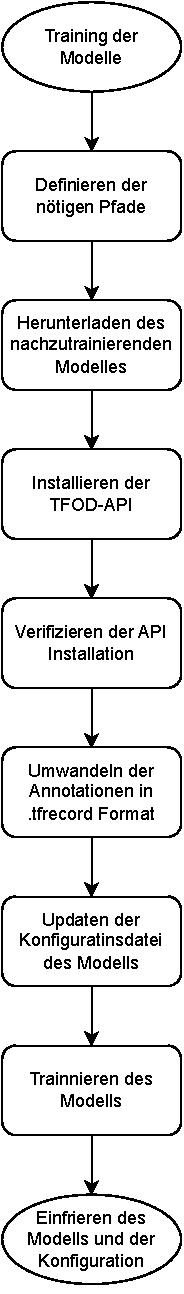
\includegraphics[width=0.18\textwidth]{images/pap_train_tensorflow.pdf}
    \label{fig:tens-pap}
    \caption{\acs*{PAP} TensorFlow Nachtraining}
\end{wrapfigure}

Bevor das Training beginnen kann, müssen die Annotationen, die in der Trainings-CSV-Datei enthalten sind, in das TFRecord-Format umgewandelt werden. TensorFlow bietet hierfür ein Python-Skript an. Allerdings musste dieses Skript angepasst werden, da es nicht direkt verwendet werden konnte. Das angepasste Skript iordnest unter dem Skriptordner enthalten.\\
Anschließend wird die Konfigurationsdatei des zuvor heruntergeladenen Modells aktualisiert. Dies bedeutet, dass die Pfade zu den Bilddaten und der TFRecord-Datei angepasst werden müssen. Darüber hinaus können weitere Trainingsparameter geändert oder hinzugefügt werden. Zum Beispiel können auch Augmentierungen hinzugefügt werden und die Anzahl der Objekttypen kann an den Anwendungsfall angepasst werden.

Erst nach Abschluss dieser Schritte kann das Training gestartet werden. Die Installation der TensorFlow Object Detection API sollte jedoch nur einmal erforderlich sein. Für das Training wird dann nur noch die Anzahl der Trainingsschritte benötigt. Diese gibt an, wie lange und intensiv das Modell nachtrainiert werden soll. Basierend auf der angepassten Konfigurationsdatei wird das Nachtraining gestartet.

Nach Abschluss des Trainings wird das Modell eingefroren. Das eingefrorene Modell kann dann für die Objekterkennung verwendet werden.

\subsubsection{Training für Google Coral} \label{cap:coral_train}

Da es nicht von Anfang an möglich war, einen Jetson Nano mit integrierter Grafikkarte zu erhalten, wurde zunächst der Ansatz mit dem Raspberry Pi verfolgt. Es war jedoch von Anfang an klar, dass die Ausführung der Objekterkennung auf dem Raspberry Pi nur zu einer geringen Anzahl von FPS führen würde. Daher war zusätzliche Hardware erforderlich, um eine Objekterkennung auf dem Raspberry Pi zu ermöglichen.
\\
In diesem Fall kommt Googles USB-Accelerator \textit{Coral} zum Einsatz. Die über USB anschließbare Edge-TPU ist speziell für KI-Inferenzanwendungen entwickelt worden. Mit seiner Hardware ermöglicht der USB-Stick die Ausführung von \ac{ML}-Algorithmen auf Geräten mit begrenzter Rechenkapazität. Der Coral USB-Stick ist in der Lage, die Objekterkennung in Echtzeit durchzuführen. Dank seines geringen Stromverbrauchs von zwei Watt und seiner Mobilität eignet sich der Coral USB-Stick auch für die Anwendung in dem Abschrecksystem. \cite{coral_google}

Auf der Coral-Webseite (\cite{coral_google}) werden ebenfalls eigene Trainingsmodelle und Jupyter-Notebooks zur Verfügung gestellt, um das Training durchzuführen. Zusätzlich wird eine Auflistung angeboten, wie die Modelle auf der Edge-TPU performen.
\\
Coral greift dabei auf Modelle von TensorFlow Version 1 und 2 zurück. Allerdings ist die Auswahl deutlich eingeschränkter als bei TensorFlow ihren \textit{Model Zoo}. Coral selbst bietet nur ein Notebook für die Nutzung mit TensorFlow Version 2 an. Weitere Notebooks sind für TensorFlow Version 1 ausgelegt. Da weder Colab noch die über den JupyterHub der DHBW zur Verfügung gestellte GPU TensorFlow Version 1 unterstützen, konnte nur dieses eine Modell getestet werden. Das Modell benötigte die Annotationen im PASCAL-VOC-Format. Dies ist das ursprüngliche Format der Waschbärbilder von Dat Tran. Unter dem Skriptordner wurde daher ein weiteres Rust-Programm entwickelt, um die CSV-Datei in XML-Dateien zu konvertieren.
\\
Um nun mehrere Modelle und deren Performance vergleichen zu können, müssen das \textit{MobileNet}-Modell von TensorFlow und das \ac{YOLO}-Modell für die Edge-TPU konvertiert werden. Bei \ac{YOLO} muss dafür nur der Exportbefehl mit dem Argument \verb|format=edgetpu| aufgerufen werden. Die Konvertierung war jedoch zunächst erfolglos. Richard Aljaste hat den Grund dafür in einem GitHub-Issue unter \cite{coral_yolo} gefunden und einen Pull Request mit einer Lösung erstellt. Dieser Pull Request wurde jedoch noch nicht in das offizielle \ac{YOLO}-Repository aufgenommen.
\\
Die Veröffentlichung des Pull Requests erfolgte Ende März und war erst im April ausgereift genug, um angewendet zu werden. Die daraus resultierende Ergebnisse können in \ref{cap:Benchmarks} eingesehen werden.

Die Konvertierung aus TensorFlow heraus verlief jedoch erfolglos. Auf ihrer GitHub-Seite wird dieses Problem immer wieder gemeldet. Es scheint, dass die für die Edge-TPU erforderliche Integer-8-Quantisierung wiederholt Schwierigkeiten verursacht. Das Modell wird dabei zwar konvertiert, aber anscheinend können die Enden der Modellarchitektur nicht immer korrekt quantisiert werden. Dies führt zu einer Senkung der Zuversichtlichkeit der Objekterkennung auf unter 5 Prozent und auch die Position der Bounding Boxes wird inkorrekt. Daher kann das Model nicht mit der Integer-8 Quantifizierung verwendet werden.

\subsubsection{\ac{YOLO}v8} \label{cap:yolov8}

Das Framework \textit{Ultralytics} ermöglicht durch einen High-Level Zugriff ein schnelles und einfaches trainieren von Klassifikations-, Segmentierungs- und Objekterkennungsmodellen. Es basiert auf dem \textit{pytorch}-Framework, das bereits einen High-Level-Zugriff auf \ac{ML}-Modelle und deren Entwicklung ermöglichte. Ultralytics vereinfacht diesen Prozess noch weiter. Für das Training werden neben den Daten nur noch die Pfade, eine YAML-Datei und der zu trainierende Modelltyp benötigt.
\\
Durch den High-Level-Zugriff wird das Deployment auf sämtlichen Plattformen ermöglicht. Mit einem einfachen Exportbefehl kann das trainierte Modell für gängige Frameworks wie TensorFlow, TensorFlow-Lite, PyTorch und ONNX konvertiert und in diesen verwendet werden.
\cite{ultralytics}

Da das Training zunächst für TensorFlow vorgesehen war, mussten die Bildannotationen von der CSV-Datei in das für das Framework geeignete TXT-Format konvertiert werden. Hierfür wurde ein selbstgeschriebenes Python-Skript im Skriptordner abgelegt.

\subsubsection{Das Training auf \textit{Google Colab}}

Für das Training der Modelle wurde zunächst \textit{Google Colab} verwendet, jedoch ist die kostenlose \ac{GPU} dort nicht besonders leistungsstark. Zudem ist die maximale Trainingsdauer auf wenige Stunden begrenzt. Colab beendet sämtliche laufende Prozesse spätestens nach zwölf Stunden und entzieht vorher die kostenlose \ac{GPU}. Darüber hinaus werden Prozesse nach zehn bis zwanzig Minuten Inaktivität beendet. Um als aktiv zu gelten und die Trainingsdauer zu verlängern, wurde ein Python-Skript entwickelt, das alle paar Minuten einen Mausklick simuliert. Dadurch kann die Trainingsdauer verlängert werden, ohne dass man aktiv am Training teilnehmen muss.erlängert werden, da man nicht aktiv beim Training etwas tun muss.
\\
Zudem mussten die Bild- und Annotierungsdaten auf Colab hochgeladen werden. Glücklicherweise verfügt Colab über eine Integration von \textit{Google Cloud}, wodurch die Bilddaten in der Cloud gespeichert und für mehrere Sitzungen verwendet werden konnten. Andernfalls müssten die Daten bei jeder Sitzung erneut hochgeladen werden, da sie bei Beendigung einer Sitzung gelöscht werden, sofern sie nicht in der Cloud gespeichert sind. Außerdem wurde festgestellt, dass bei wiederholter hoher Auslastung während einer Sitzung die Zeit bis zur Sitzungsbeendung durch Colab weiter verkürzt wird. Ein effektives Training von Modellen ist dadurch nicht möglich.

Zu einem späteren Zeitpunkt konnte die DHBW über den eigenen JupyterHub eine leistungsstarke GPU zur Verfügung stellen. Mit dieser konnte die maximale Trainingszeit von wenigen Stunden auf mehrere Tage ausgedehnt werden. Zudem verkürzte sich die Trainingszeit von einigen Stunden auf weniger als 30 Minuten, was zu einem erheblichen Leistungssprung führte.

Allerdings hatte der Wechsel seine Nachteile. Aufgrund unzureichender Berechtigungen zur Installation aller benötigten Bibliotheken - TensorFlow (Objekterkennungs-API), Edge-TPU-Konvertierung und TensorFlow-Lite Model Maker (Google Coral) - war es nur noch möglich, \ac{YOLO}-Modelle zu trainieren.

\subsection{Deployment}

Für das Deployment wurden verschiedene Modelle und Laufzeitumgebungen erstellt. Daher war es erforderlich, fünf Laufzeitumgebungen einzubinden bzw. zu unterstützen, um die Modelle auswerten zu können. Nachfolgend sind die einzelnen Umgebungen beschrieben. Die verschiedene Ergebnisse bei der Nutzung der Umgebungen werden in Kapitel \ref{cap:Benchmarks} beschrieben.

\subsubsection{TensorFlow}

TensorFlow speichert seine Dateien als .pb-Dateien ab, die mit der normalen TensorFlow-API in das Programm geladen werden können. Eine Installation der Object Detection API ist nur für das Training der Modelle erforderlich.
\\
Anschließend muss das Eingabebild an das Modell angepasst werden. Wenn das Bild zu groß ist, z.B. mit einer 4K-Auflösung, muss es zuerst verkleinert werden. Außerdem benötigen alle Bilder eine zusätzliche Dimension. Diese Dimension kann einfach mit dem \verb|expand_dims|-Befehl von NumPy hinzugefügt werden.
\\
Danach kann das Bild dem Modell zur Verarbeitung übergeben werden. \cite{tens_zoo}

Die Ausgabe der TensorFlow-Modelle muss dennoch nachbearbeitet werden, da sie alle Erkennungen bis zur eingestellten maximalen Anzahl ausgibt. Bei der Standardkonfiguration von MobileNet wären das bis zu 100 Erkennungen. Um unerwünschte Erkennungen herauszufiltern, z.B. solche mit einer Zuversichtlichkeit von nur 1\%, wird die Ausgabe gefiltert und in ein Dictionary gespeichert.

Damit ist die Erkennung mittels der TensorFlow API abgeschlossen und die Ausgabewerte können vom Hauptprogramm ausgewertet werden.

\subsubsection{TensorFlow-Lite und Google Coral}

Die TensorFlow Lite-Umgebung basiert auf TensorFlow. TensorFlow Lite-Modelle sind jedoch kompakter als die .pb-Modelle von TensorFlow. Allerdings erfordern sie mehr Aufwand für die Initialisierung von Modellen, da beim Laden des Modells explizit das Format der Ein- und Ausgabeparamter aus dem Modell geladen werden müssen. Diese werden anschließend in der Ausführung und Nachbearbeitung verwendet.
\\
Ein Vorteil gegenüber den TensorFlow-Modellen besteht darin, dass sie besser für die Ausführung auf einer CPU geeignet sind. Dies liegt darin, dass sie eine geringere Rechenintensität besitzen. TensorFlow bietet drei Quantisierungstyps dafür an: Float-32, Float-16 und Integer-8.
\\
Die Bezeichnungen beschreiben die Art der Gradientenoptimierung. Während Float-32 und -16 Gleitkommazahlen beschreiben, trifft dies bei Integer-8 nicht zu. Bei Integer-8 handelt es sich um eine Ganzzahl im Bereich von 0 bis 255. Die Zahlen 8, 16 und 32 geben die Anzahl der Bits an, mit denen ein Gradient gespeichert wird. Das Modell hat also den kleinsten Speicherbedarf wenn eine Integer-8 Quantifizierung der ursprünglichen .pb-Modelle vorgenommen wird.
\\
Die Wahl des Quantisierungstyps hängt dabei von den spezifischen Anforderungen und den verfügbaren Ressourcen ab. Float-32 bietet die höchste Genauigkeit, benötigt jedoch mehr Speicherplatz und kann mehr Ausführungszeit benötigen. Float-16 bietet eine gute Balance zwischen Genauigkeit und Ressourcenverbrauch. Integer-8 hat den geringsten Speicherbedarf und kann auf Hardwareplattformen mit geringerer Präzision wie Mikrocontrollern effizienter ausgeführt werden.
\\
Bei der Quantifizierung der Modelle treten allerdings auch Genauigkeitsverluste auf. Dieser Verlust könnte unter Umständen nicht im toleranten Bereich der Anwendung sein. Im Kapitel \ref{cap:Benchmarks} werden auch diese Verluste genauer betrachtet.
\cite{tens_zoo}

Auf dem USB-Accelerator Coral können allerdings nur Integer-8 Quantifizierte Modelle betrieben werden. Die anderen Modelle werden daher auf der CPU des Mikrocontrollers ausgeführt. Um den USB-Accelerator nutzen zu können muss allerdings lediglich der TensorFlow-Lite Umgebung dies mitgeteilt werden. \cite{coral_google}

\subsubsection{ONNX}

Um Objekterkennungsmodell im ONNX-Format auf dem Jetson nutzen zu können gibt es drei Möglichkeiten: OpenCV, ONNX-Runtime und TensorRT. TensorRT wird im nachfolgenden Kapitel beschrieben, da hierzu weitere Schritte nötig sind.

Das ONNX-Format wird für die Nutzung der \ac{YOLO}-Modelle verwendet. Die trainierten \ac{YOLO}-Modelle können durch das Ultralytics-Framework direkt exportiert und verwendet werden. Laut Ultralytics ermöglicht das konvertieren des Modells nach ONNX eine bis zu dreimal schnellere Ausführungszeit. \cite{ultralytics}
\\
Exportierte Modelle können auch direkt mit dem Ultralytics-Framework verwendet werden. Dabei gab es jedoch Probleme mit PyTorch, auf dem das Ultralytics-Framework basiert.
\\
Das Ultralytics-Framework kann zwar manuell über die Quelldateien auf dem Jetson Nano installiert werden, aber es treten bei der Ausführung Probleme. Um das Framework nutzen zu können, muss zusätzlich zu PyTorch die \textit{torchvision}-Bibliothek installiert werden. Während dem Detektieren von Objekten trat das Problem auf, da das Detektieren von Objekten nur solange funktionierte nur solange, bis ein Objekt erkannt wurde. Sobald ein Objekt erkannt wurde, kam es zu einer Fehlermeldung. Diese besagt, dass nicht die richtige Version von \textit{torchvision} installiert wurde, da sie nicht mit PyTorch kompatibel sei.
\\
Das Nvidia-Forum enthält mehrere Einträge zu diesem Thema. Das eigene Nvidia-Forum, dass die Installation von PyTorch und torchvision beschreibt, enthält über 1200 Einträge mit vielen Lösungsmöglichkeiten. Allerdings konnten viele davon das Problem nicht lösen, wodurch das nutzen des Frameworks auf dem Jetson Nano für das Abschrecksystem nicht möglich war. \cite{pytorch_jn}

OpenCV verfügt ebenfalls über die Möglichkeit, ONNX-Modelle zu laden und eine Objekterkennung durchzuführen. Allerdings müssen die Bilddaten vorher mit der Funktion \verb|blobFromImage| vorbereitet werden, um sie für die Verarbeitung dem Modell übergeben zu können.
\\
Nachdem das Modell die Bilddaten verarbeitet hat, muss die Ausgabe nachbearbeitet werden. Dabei werden zunächst die Zuversichtlichkeiten der Bounding Boxen extrahiert und überprüft, ob dieser Wert ausreichend hoch ist. Diese Nachbearbeitung ist ähnlich wie bei TensorFlow. Allerdings konnte bei TensorFlow direkt über ein Dictionary auf die Zuversichtlichkeit zugegriffen werden. Beim ONNX-Format muss diese zunächst durch das Auswählen der entsprechenden Ausgabewerte extrahiert werden. Gleiches gilt für die Ermittlung der Bounding Boxen. \cite{opencv_onnx}
\\
Ein ähnliches Verfahren wird bei der Verwendung der ONNX-Runtime angewendet. Der Unterschied zwischen den beiden liegt jedoch in der Ausführungszeit. Die ONNX-Runtime verarbeitet die Eingabewerte schneller als OpenCV, wie aus den Ergebnissen in Kapitel \ref{cap:Benchmarks} hervorgeht.

\subsubsection{TensorRT} \label{cap:tensorrt}

TensorRT ist eine Optimierungs- und Inferenz-Laufzeitbibliothek, die von Nvidia für ihre Grafikkarten entwickelt wurde. Der Zweck dieser Bibliothek besteht darin, \ac{DNN}s für den Einsatz auf Nvidia-GPUs zu optimieren und die Ausführungszeit zu reduzieren. Dafür benötigt die Bibliothek bereits trainierte Modelle von TensorFlow oder PyTorch. Anschließend werden auf diesen Modellen eine Reihe von Optimierungen durchgeführt, um die Inferenzgeschwindigkeit und -effizienz zu verbessern, ohne die Genauigkeit der Modelle zu beeinträchtigen. \\
Um diese Optimierungsmöglichkeit nutzen zu können, müssen bestehende Modelle in das ONNX-Format konvertiert werden. PyTorch-Modelle können ohne weiteres Zutun direkt in das ONNX-Format konvertiert werden. Für die Verwendung von TensorFlow-Modellen muss jedoch ein Zwischenschritt über die Bibliothek \textit{tf2onnx} erfolgen. Es kann auch erforderlich sein, das exportierte Modell im ONNX-Format zu bearbeiten, falls Probleme bei der Optimierung des Modells auftreten.
\cite{Tensorrt_2023_nvidia}

Wie auch bei TensorFlow mit TensorFlow-Lite gibt es auch hier die Möglichkeit, die Quantisierung auf Float-32, Float-16 oder Integer-8 festzulegen. Das ermöglicht die Reduzierung des Speicherbedarfs und die Verbesserung der Inferenzgeschwindigkeit auf den Nvidia-\ac{GPU}s, sowie dem Jetson Nano.

Es ist möglich, die mit TensorRT optimierten Modelle sowohl mit TensorRT als auch mit PyTorch zu verwenden. Es wird sogar in \cite{mu_tensorrt} empfohlen, TensorRT in Kombination mit PyTorch zu nutzen, da es performanter sein kann.
\\
Diese Möglichkeit kann jedoch aufgrund der bereits genannten Versionsprobleme derzeit nicht angewendet werden.
Daher wurde die alternative Methode getestet, nämlich die Verwendung von TensorRT mit PyCuda. Dabei müssen die Eingabe- und Ausgabewerte manuell mit PyCuda gesetzt bzw. gelesen werden. Zusätzlich ist mehr Initialisierungscode erforderlich. Durch anfängliche Fehler bei der Konfiguration dieses Codes kam es daher zu keiner sinnvollen Ausgabe. Diese Probleme konnten jedoch im Nachhinein behoben werden.

Die Vorbereitung der Bilddaten und die Nachbearbeitung der Ausgabe sind nahezu identisch zur Verwendung des ONNX-Formats. Der einzige Unterschied besteht darin, dass die Ausgabe in einer anderen Form vorliegt und daher ein anderes Slicing benötigt wird.


\subsection{Auswertung der Modelle auf ihre Eignung für das Abschrecksystem} \label{cap:Benchmarks}

Da für den Einsatz im Abschrecksystem das Modell präzise und effizient Arbeiten muss folgt eine detaillierte Auswertung der verschiedenen Modelle hinsichtlich ihrer Eignung für das Abschrecksystem. Dabei werden die Modelle auf Basis ihrer Infrenzzeit und Zuversichtlichkeit analysiert und miteinander verglichen. Im Folgenden werden die Ergebnisse und Erkenntnisse dieser Auswertung präsentiert.

\subsubsection{Inferrenzzeit der Modelle}

Ein wichtiger Aspekt ist die Inferenzzeit, die entscheidend dafür ist, Tiere in Echtzeit erkennen zu können. Daher wurden die Modelle auf verschiedenen Hardwareplattformen getestet, um die Leistung in Bezug auf die Inferenzzeit zu bewerten. Es wurden signifikante Unterschiede sowohl aufgrund der Hardware als auch aufgrund des Modellformats festgestellt. Ein Auszug der Ergebnisse ist in Tabelle \ref{tab:bench_time} dargestellt.

\begin{table}[h]
    \resizebox{\textwidth}{!}{%
    \begin{tabular}{|l|llccc}
        \textbf{Modell} & \textbf{Hardware} & \textbf{Format} & \textbf{Schlechtester Lauf} & \textbf{Bester Lauf} & \textbf{Durchschnitt}\\
        \hline
        MobilNet SSD & I7-10th & pb  & 147 & 26 & 52 \\
        MobilNet SSD & I7-10th & TFLITE-f32 & 106 & 18 & 39 \\
        MobilNet SSD Treaded & I7-10th & TFLITE-f32 & 71 & 0 & 21 \\
        MobilNet SSD Treaded & I7-10th & TFLITE-f16 & 37 & 0 & 17 \\
        MobilNet SSD & Jetson & pb  & 681 & 104 & 111 \\
        MobilNet SSD Treaded & Jetson & TFLITE-f16 & 675 & 0 & 113 \\
        YOLOv8n & I7-10th & pb & 47 & 13 & 17 \\
        YOLOv8n Treaded & I7-10th & TFLITE-f32 & 37 & 0 & 15 \\
        YOLOv8n Treaded & I7-10th & TFLITE-f16 & 31 & 0 & 13 \\
        YOLOv8n Treaded & I7-10th & TFLITE-i8 & 28 & 0 & 12 \\
        YOLOv8n & Jetson & pb  & 82 & 48 & 53 \\
        YOLOv8n Treaded & Jetson & TFLITE-f32 & 226 & 166 & 179 \\
        YOLOv8n OpenCV & Jetson & ONNX & 47 & 41 & 42 \\
        YOLOv8n ONNX & Jetson & ONNX & 43 & 33 & 39 \\
        YOLOv8n TensorRT & Jetson & ONNX & 16 & 10 & 13 \\
        YOLOv8n Treaded & CM3 & TFLITE-f32 & 686 & 559 & 591 \\
        YOLOv8n & CM3 + Coral & TFLITE-i8  & 89 & 63 & 68 \\
        YOLOv8n & Jetson + Coral & TFLITE-i8  & 20 & 16 & 17 \\
        YOLOv5n & I7-10th & pb & 75 & 13 & 26 \\
        YOLOv5n & Jetson & pb & 70 & 43 & 47 \\
        EfficientDet D0 & I7-10th & pb & 453 & 183 & 249 \\
        EfficientDet D0 & Jetson & pb & 1623 & 492 & 511 \\
    \end{tabular}
    }
    \caption{Vergleich verschiedener Objekterkennungsmodelle auf Basis ihres Formates und Inferennzzeit in Millisekunden}
    \label{tab:bench_time}
\end{table}

In der Tabelle ist ein Ausschnitt der durchgeführten Inferenzmessungen zu sehen. Zunächst wurde das Modell \textit{MobileNet} von TensorFlow getestet. Der Test wurde auf einem Laptop mit einem Intel i7-Prozessor der zehnten Generation durchgeführt. Dabei wurde festgestellt, dass das Modell durch die Quantisierung erheblich beschleunigt wurde. Die Verwendung der Float-16-Quantisierung führte zu einer Reduzierung der Ausführungszeit auf ein Drittel der ursprünglich benötigten Zeit. Die Beschleunigung war auch Multithreading zu verdanken. In der TensorFlow-Lite-Umgebung kann man nämlich die Anzahl an Threads, die dem Prozess zustehen, erhöhen. Durch die eingestellten vier Treads konnte daher ebenfalls eine Verringerung der Ausführungszeit ermöglicht werden, wie an dem Float-32 quantifizierten Modell zu erkennen ist.
\\
Als derselbe Test auf dem Jetson durchgeführt wurde, konnte nicht die gleiche Beschleunigung beobachtet werden. Dies liegt daran, dass die TensorFlow-Umgebung auf die GPU zugreifen kann, während die TensorFlow-Lite-Umgebung dies nicht kann. Das quantisierte Modell läuft daher auf der CPU des Jetsons, was zu einer deutlichen Steigerung der Inferenzzeit führt. Deshalb haben das ursprüngliche Modell und das float-32-quantisierte Modell nahezu die gleiche durchschnittliche Ausführungszeit von 100 Millisekunden. Eine Inferenzzeit in diesem Bereich ermöglicht keine Echtzeit-Erkennung der Tiere, weshalb eine weitere Untersuchung des Modells nicht länger in Betracht gezogen wurde.

Das zweite TensorFlow-Modell, das \textit{EfficientDet D0}, wurde ebenfalls verworfen. Aufgrund seiner höheren Auflösung lag die Ausführungszeit auf dem Jetson bei über 500 Millisekunden, was für das Abschrecksystem nicht geeignet ist. Die Möglichkeit, die Modelle in das ONNX-Format zu konvertieren und dadurch eine potenzielle Verbesserung der Ausführungszeit zu erzielen, wurde jedoch nicht getestet. Diese Entscheidung wurde aufgrund der Erkenntnisse aus Kapitel \ref{cap:qual_erk}, die parallel gewonnen wurden, getroffen.
\\
Durch diese Erkenntnisse sind nur noch die \ac{YOLO}-Modelle in Frage gekommen. 

Auch beim YOLOv8-Modell zeigt sich das gleiche Verhalten wie beim MobileNet-Modell. Auf dem Intel I7-Prozessor wird die Ausführungszeit durch die Quantifizierung stark beschleunigt, jedoch nicht auf dem Jetson. Da aber die Integer-8-Quantifizierung funktioniert, konnte die Ausführungszeit auf dem USB-Accelerator Coral in Kombination mit dem Raspberry Pi CM3 und dem YOLO-Modell getestet werden.
\\
Mit einer durchschnittlichen Ausführungszeit von 68 Millisekunden im Vergleich zu den 17 Millisekunden auf dem Jetson, war das Ergebnis aber eher ernüchternd.Deshalb wurde das Raspberry Pi CM3 endgültig von der Liste der möglichen Mikrocontroller für den Einsatz im Abschrecksystem gestrichen. Der Grund für den extremen Unterschied liegt allerdings am USB-Anschluss des CM3. Das CM3 verfügt nämlich nur über einen USB 2.0-Port, während der Jetson Nano über USB 3.0-Ports verfügt. Dadurch geht der Datenaustausch zwischen dem Mikrocontroller und dem Coral USB-Stick beim Raspberry Pi CM3 langsamer vonstatten.

Das Ultralytics-Framework bot auch die Möglichkeit, ältere YOLO-Modelle wie das YOLOv5-Modell zu trainieren. Dieses Modell wurde ebenfalls kurz getestet, jedoch wurde kein Vorteil gegenüber dem neueren YOLOv8-Modell festgestellt. Daher wurde dem YOLOv5-Modell keine weitere Beachtung geschenkt.

Somit blieb nur noch die Konvertierung in das ONNX- und TensorRT-Format als Option übrig. Das mit TensorRT konvertierte Modell erreichte eine beeindruckende Ausführungszeit von 13 Millisekunden für die Verarbeitung der Eingabewerte. Allerdings ist bei genauerer Untersuchung das Problem aus Kapitel \ref{cap:tensorrt} bemerkt worden. Die Verwendung von PyCuda in Verbindung mit der Vor- und Nachbearbeitung verschlechterte die Ausführungszeit erheblich. Dadurch erreichte das TensorRT-Modell letztendlich eine ähnliche Ausführungszeit wie das ONNX-Runtime-Modell. Allerdings war der Ressourcenverbrauch des TensorRT-Modells deutlich höher. Nahezu alle vier Kerne und die \ac{GPU} liefen bei dem Inferenztest auf der maximalen Leistung. In der ONNX-Runtime war der Verbrauch etwas geringer, weshalb dieses Modell eher für die Verwendung im Abschrecksystem geeignet war.

\subsubsection{Zuversichtlichkeit der Modelle} \label{cap:qual_erk}

Ob die Modelle jedoch für das Abschrecksystem geeignet sind, hängt nicht allein von der Inferenzzeit ab, sondern auch von der Qualität des Modells selbst ab. Diese beschreibt, wie gut das Modell mit Daten aus der realen Welt zurechtkommt, das heißt, ob und wie gut das Modell die Tiere erkennen kann.

Hierbei kommt die in Kapitel \ref{cap:struktur} beschriebene Ordnerstruktur zum Tragen. Ein Teil der gesammelten Bilder wurde bereits von den für das Training des Modells vorgesehenen Daten getrennt. Diese Bilder bilden das Testset.
\\
Während des Trainings lernt das Modell Erkennungsmethoden anhand des Trainingssets und überprüft deren Genauigkeit anhand der Daten im Devset. Das Testset bleibt dabei völlig unbekannt und kann daher für eine grobe Abschätzung der Performanz auf unbekannte Daten verwendet werden.

Dafür wird der \acf{mAP} der Modelle ermittelt. Diese ist eine  Bewertungsmetrik, die häufig zur Evaluierung von Objekterkennungssystemen verwendet wird. Dabei wird gemessen, ob die erkannten Objekte tatsächlich korrekt sind. Dabei können die Bounding Boxen auch bis zu einen gewissen Grad schwanken ohne den \ac{mAP} zu verschlechtern. Dadurch kann eine umfassende Bewertung der Modellleistung durchgeführt werden. \cite{cv_Szeliski}

Um diesen Wert zu bestimmen, wird in TensorFlow das Programm TensorBoard verwendet. Mit diesem Tool kann die mittlere durchschnittliche Präzision (\ac{mAP}) zu jedem Trainingszeitpunkt abgerufen werden. Standardmäßig wird jedoch nur beim letzten Schritt nach dem Training die Evaluierung durchgeführt.
\\
Daher ist in Abbildung \ref{fig:map_Mobilnet} die Präzision erst nach 50.000 Trainingsschritten dargestellt. Die aus den Daten entnommene \ac{mAP} für die Präzesion der Bounding Boxen im mittleren Bereich liegt demnach bei 36\%.

Beim Ultralytics-Framework wird ebenfalls eine ähnliche Art der Evaluation durchgeführt. Dabei erfolgt standardmäßig nach jeder Trainingsepoche eine Auswertung. Die Ergebnisse der Evaluation werden dem Entwickler nach jeder Epoche mitgeteilt. Zudem erstellt das Ultralytics-Framework automatisch ein Diagramm, das den Verlauf der mittleren durchschnittlichen Präzision (\ac{mAP}) über die einzelnen Trainingsepochen anzeigt. Dadurch ist es nicht erforderlich, ein zusätzliches Tool zu installieren. Es werden auch weiter Metriken, wie z.B. den F1-Wert berechnet. Daher bietet das Framework eine schnelle und aussagekräftige Auswertung des Modells.

\begin{figure}[H]
    \centering
    \begin{minipage}{0.48\textwidth}
        \centering
        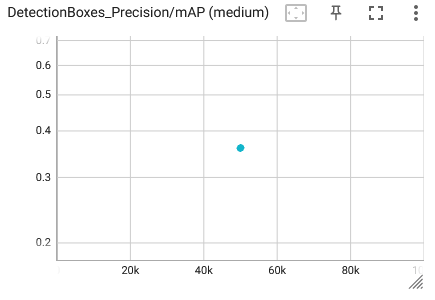
\includegraphics[height=5cm]{images/mobileNet_map.png}
        \caption{\ac{mAP} des MobileNet-Modells nach 50.000 Trainingsschritten}
        \label{fig:map_Mobilnet}
    \end{minipage}
    \hfill
    \begin{minipage}{0.48\textwidth}
        \centering
        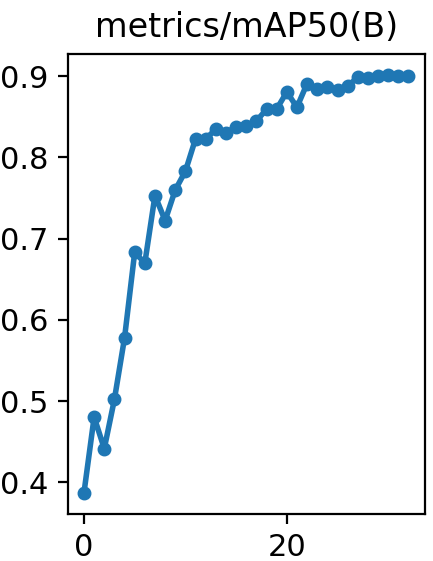
\includegraphics[height=5cm]{images/P_curve.png}
        \caption{\ac{mAP} des YOLOv8-Modells nach 30 Epochen}
        \label{fig:map_yolo}
    \end{minipage}
\end{figure}

Aus den Daten in den Abbildungen \ref{fig:map_Mobilnet} und \ref{fig:map_yolo} lässt sich ableiten, dass das YOLO-Modell deutlich schneller eine höhere Präzision erreicht hat. Daher wurde weiterhin mit dem \ac{YOLO}-Modell gearbeitet.

Beim Vergleich wurde darauf geachtet, dass die Modelle einen ähnlichen Ressourcenverbrauch während des Trainings aufweisen. Beide Modelle wurden für etwa dreieinhalb Stunden auf Google Colab trainiert. Bei gleicher Batch-Größe benötigte das MobileNet-Modell jedoch mehr RAM als das Konkurrenzmodell.

Aus der Auswertung dieser Untersuchung geht hervor, dass das YOLOv8-Modell als Basismodell verwendet werden sollte, da es die Anforderungen an das Abschrecksystem am besten erfüllt.
\\
Da beim Konvertieren und Quantifizieren der Modelle eine Verringerung des \ac{mAP}-Werts auftreten kann, wurden diese ebenfalls überprüft. Die konvertierten und quantifizierten Modelle können direkt in das Ultralytics-Framework geladen werden, was den Auswertung gegenüber der TensorFlow Modelle vereinfacht. Bei TensorFlow gibt es diese Möglichkeit nämlich nicht direkt. Ein Vergleich der Ergebnisse kann in Tabelle \ref{tab:map_yolo} eingesehen werden.

\begin{table}[h]
    \centering
    \begin{tabular}{llcc}
        \textbf{Format} & \textbf{Quantifizierung} & \textbf{\ac{mAP}-50} & \textbf{\ac{mAP}-50}\\
        \hline
        pt & - & 95,5 & 76,5\\
        TFLITE & Float-32 & 88,9 & 66,4 \\
        TFLITE & Float-16 & 88,9 & 66,4\\
        TFLITE & Integer-8 & 76,4 & 51,6\\
        ONNX & - & 92,3 & 71,8\\
    \end{tabular}
    \caption{Vergleich des \ac{mAP}-Wertes verschiedener YOLOv8-Quantifizierung und Modellformate}
    \label{tab:map_yolo}
\end{table}

Daraus geht hervor, dass die Integer-8-Quantifizierung eine erhebliche Verschlechterung des \ac{mAP}-Werts verursacht. Angesichts dessen wird die Verwendung von Integer-8-quantifizierten Modellen verworfen.
\\
Beim Anwenden der Quantifizierung auf das ONNX-Modell wird ein ähnliches Verhalten beobachtet. Da das Modell jedoch auch für die Verwendung von TensorRT vorgesehen ist, wird eine weitere Quantifizierung nicht verwendet. TensorRT bietet die Möglichkeit, zu bewerten, ob ein Knoten mit Integer-8 quantisiert werden soll. Dabei wird darauf geachtet, ob ein Präzisionsverlust durch die Quantifizierung auftritt. Diese automatische Auswahl der besten Optimierung des Modells ermöglicht die kürzeste Inferenzzeit bei vernachlässigbarem Präzisionsverlust.

Im Anschluss an diese Auswertung wurden zudem mehrere Testmodelle mit unterschiedlichen Augmentierungen erstellt. Diese Augmentierungen sollten die Modelle besser auf den Einsatz im Abschrecksystem abstimmen. Die Problematik wurde bereits in Kapitel \ref{cap:augment} beschrieben.
\\
Anschließend wurden die Modelle anhand einer handverlesenen Auswahl von Bildern getestet. Durch die Augmentierung ist zwar der \ac{mAP}-Wert, der auf den Online-Datensätzen angewendet wurde, gesunken, aber die Erkennung der Tiere auf den ausgewählten Bildern wurde deutlich verbessert.

\section{Zusätzliche Softwarekomponenten}

Für das Abschhrecksystem sind zusätzliche Softwarekomponnenten von nöten. Die wichtigsten werden folgend beschrieben.

\subsection{Erkennung durch Kontur-tracking}

\subsection{Verbesserung der Bildqualität}

\subsection{Tiefenberechnung} \label{cap:calc_depth}

\subsection{Kombination der Softwarekomponenten}
Auch mit random 0 Byte Bilddaten/ fehlende XML-Dateien /leere XML-Dateien und das diese für weiteres Training verwendet werden können. Warum XML? Konvertierungsskript vorhanden, sowie falls 0 Byte Fehler wärs bissle schaud für der rest, weil die dann au weg wäred

\section{Kostenaufstellung}

Folgend sind die Kosten und Verwendungszwecke aufgelistet. 

\begin{longtable}{ p{0.15\textwidth}|p{0.2\textwidth}|p{0.5\textwidth} }
    \endfirsthead
    \multicolumn{2}{l}%
    {\textit{Fortsetzung von vorheriger Seite}} \\
    \hline
    \endhead
    \hline \multicolumn{2}{r}{\textit{Fortsetzung auf nachfolgender Seite}} \\
    \endfoot
    \endlastfoot
    \textbf{Bauteil} & \textbf{Gesamtpreis in € (inkl. Mwst.)} & \textbf{Beschreibung}\\
    \hline
    LED-Scheinwerfer
    & \centering11.99
    & Die effizienten LED-Scheinwerfer sind für die Anwendung als Erweiterungsleuchten für das Fahrzeug gedacht. \cite{am_licht} Da die LEDs den hohen Belastungen beim Einsatz am Fahrzeug standhält, werden sie den Anforderungen an einem portablem Abschrecksystem gerecht. Sie werden als Blitzlicht für das Abschrecksystem verwendet.
    \\
    Membran-pumpe
    & \centering73.35
    & Membranpumpen sind bei einfachen und kostengünstigen Anwendungen vertreten. Durch den geringen Verschleiß und einfache Wartbarkeit werden sie häufig in Frisch- und Abwasseranwendungen eingesetzt. \cite{mebranpumpe} In der Arbeit wird die Pumpe wegen ihrem geringen Verschleißes und Anschaffungskosten verwendet.
    \\
    Solarpanel
    & \centering69.99
    & Das Solarmodul wird verwendet um die Portabilität und Autarken Eigenschaften der Abschrecksystems zu gewährleisten. Solange Sonnenlicht am Einsatzort verfügbar ist, kann das Abschrecksystem mit ausreichend Energie versorgt werden um die unliebsamen Kleintiere zu erkennen.
    \\
    Autobatterie
    & \centering59.90
    & Kombiniert mit dem Solarmodul versorgt die Batterie das Abschrecksystem mit der nötigen Energie. Tagsüber wird sie mithilfe des Solarmoduls aufgeladen, während sie Nachts das System mit Energie versorgt. \cite{Autobatterie}
    \\
    Diverse Kleinteile
    & \centering{35 + X}
    & Diverse Kleinsteile werden in der Arbeit verwendet. Auch die Transistoren, die verwendet werden um die verschiedenen Aktoren an- und auszuschalten fallen unter dieser Kategorie. Aber auch die Räder, Schläuche, Kabel, Steckverbindungen und Schrauben werden hier miteinberechnet. Zusätzlich kommen die, für das Abschrecksystem angefertigten 3D-gedruckten Elemente hinzu.
    \\
    NOIR-Kameras
    & \centering55.98
    & In der Studienarbeit sind mehrere Kameras verbaut. Dabei wurde zunächst in hinsicht auf den Raspberry Pi, die Kamerasensoren OV5647 angeschaft worden. Diese sind allerdings nicht mit dem Jetson Nano kompaible, weshalb weitere Kamerasensoren bestellt weerden mussten. Die IMX-219 Kamerasensoren sind zudem teurer, weshalb die Kosten für die Kameras von 39.98€ auf 55.98€ erhöhte.
    \\
    Jetson Nano
    & \centering189
    &  Der Jetson Nano bildet den Kern des Abschrecksystems. Über ihn werden die Tiere erkannt und das Zielsystem und die weiteren Abschreckakoren angesteuert. Mit einer GPU ausgestattet ist sie in der Lage Echtzeiterkennung der Tiere zu ermöglichen.\newline
    Da aufgrund von Ansteuerungsproblemen der Nano nicht in der Lage war die Hardware direkt anzusteuern, musste ein Arduino UNO diese Funktion übernehmen. Dadurch entstanden zusätzliche Kosten von 13.99€\\
    Aluminium-kiste
    & \centering{109 DM}
    & Die Aluminiumkiste ist Witterungsfest und besitzt eine gute Wärmeableitung. Alle Aktoren und Gerätschaften können in ihr vor Witterungsbedingungen geschützt untergebracht werden.\\
    \caption{Kostenübersicht und Erklärung der Funktion der verschieden angeschafften Hardware}
\end{longtable}

Viele Kleinteile, sowie der Lautsprecher konnten aus dem eigenen Bestand verwendet werden. Daher wird unter dem Punkt \textit{Diverse Kleinteile} eine Summe $X$ angegeben. Die Kosten des Abschrecksystem berufen sich nach dieser rechnung auf mindestens 550€. Dabei kamen circa 200€ für das Verwenden eines autoarken Systems auf. Der Aufbau kann in Abbildung \ref{fig:whole_thing} betrachtet werden. Das 3D-Modell ermöglichte eine übersichtliche Darstellung aller Hardwarekomponenten.

\begin{figure}[H]
    \centering
    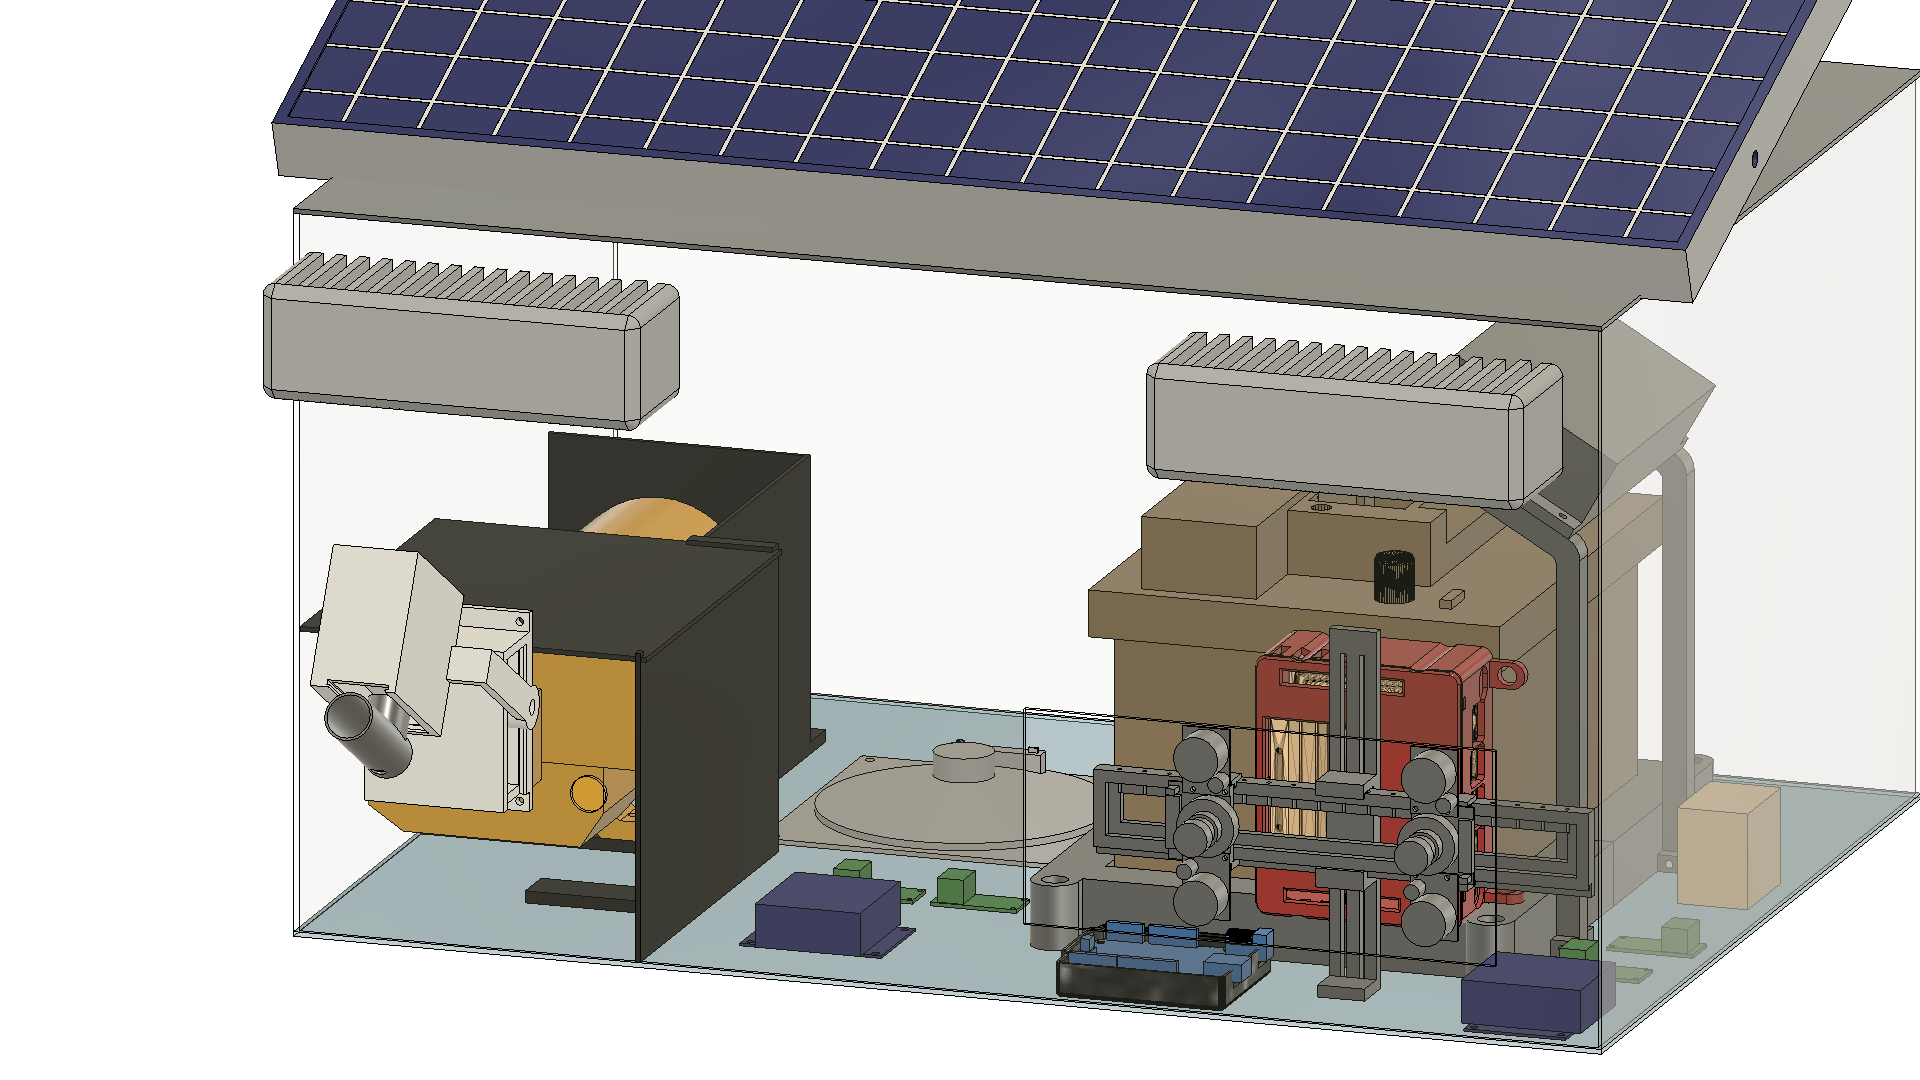
\includegraphics[width=\textwidth]{images/whole_box.png}
    \label{fig:whole_thing}
    \caption{Aufbau aller Hardwarekomponenten innerhalb eines 3D-Modells}
\end{figure}
